%************************************************
\chapter{Background on Efficient Language Models}\label{ch:efficient_lm}
%************************************************
We've discussed Transformers and how scaling them yields substantial improvements on natural language tasks.
However, scaling a Transformer-based language model is costly in terms of both training and inference
compute. In this chapter, we discuss LLM efficiency mainly through the lens of \textbf{model compression} and \textbf{activation sparsity},
since our contributions concern these two aspects. 
We present common approaches for scaling LLMs efficiently during training
and serving them efficiently during inference.

When talking about \textit{efficiency} in LLMs, there are some important concepts to know. 
The first distinction is between \textbf{compute-boundness} and \textbf{memory-boundness}.
A model or a task is compute-bound when the bottleneck is the number of arithmetic operations
that can be done per second. In that case, the limitation is not only the theoretical
peak compute of the hardware, but also how well the model and the implementation can use this compute.
A model or a task is memory-bound when the bottleneck is instead the movement of data:
loading weights, reading activations, writing tensors, or moving the KV-cache from the GPU memory.
Depending on whether we are training, doing prefill, or decoding tokens, these two concepts
do not have the same consequences. This distinction explains why diffusion-based
LLMs such as LLaDA or Gemma-Diffusion are much faster than autoregressive LLMs.
Diffusion LLMs are compute-bound and more FLOP-intensive than autoregressive LLMs.
However, their parallel decoding reduces data movement relative to autoregressive decoding
and leads to faster generation.

LLM training is mostly compute-bound, because training is highly parallel. 
Many tokens are processed at once, and the forward and backward passes are dominated by large matrix multiplications.
So the key metrics to check are \textbf{FLOPS} (how many floating-point operations are executed per second),
\textbf{MFU} (how much of the theoretical peak compute of the hardware is really used),
and \textbf{Tokens/s} (the number of tokens processed per second).
The goal is to make the model perform a lot of useful operations per second while minimizing communication:
between GPUs, between CPU and GPU, and between HBM and the compute units of the GPU. 
This is why training efficiency is not only about reducing the number of parameters.
It is also about keeping the hardware busy. We will later see that small dense models, sparse models,
and compressed models do not all use the hardware in the same way. FLOPS and MFU
are hardware-oriented numbers, so they are often complemented by \textbf{Tokens/s}, which measures
how quickly the model consumes the training data.

LLM inference can be compute-bound, but is more often memory-bound because tokens are generated one at a time.
At each decoding step, the model has to read its weights and the KV-cache to produce only one new token,
which creates a lot of memory traffic for a relatively small amount of computation.
There are two phases in LLM inference. The first is the \textbf{prefill}, where the system prompt,
the user prompt and the context are fed in parallel to the LLM. This phase is closer to training
and is often compute-bound. The second phase is \textbf{decoding}, where the model generates the text
token by token. This is usually the bottleneck, because the model repeatedly accesses the same weights
and an increasingly large KV-cache. This difference is important because a model that
requires more FLOPS can sometimes be faster if it uses the hardware better or moves less data.
The key metrics for inference follow these two phases. For prefill, we usually look at
\textbf{Time To First Token} (TTFT), which measures how long the user waits before seeing the first
generated token, and \textbf{prefill Tokens/s}, which measures how fast the prompt is processed.
These two metrics are related, but they are not exact inverses because TTFT also includes overheads
and the generation of the first token. For decoding, we look at \textbf{Time Per Output Token} (TPOT),
which measures the time needed to generate one new token, and \textbf{generated Tokens/s}, which
measures how many new tokens are produced per second. These two metrics describe the same decoding
speed with inverse units. Finally, we also care about the \textbf{memory footprint}, especially the
weights and KV-cache memory.

\begin{table*}[h!]
    \centering
    \small
    \setlength{\tabcolsep}{6pt}
    \renewcommand{\arraystretch}{1.15}
    \begin{tabularx}{\textwidth}{@{} l l >{\raggedright\arraybackslash}X @{}}
        \toprule
        \textbf{Phase}
        & \textbf{Metric}
        & \textbf{What it measures} \\
        \midrule
        \multirow{3}{*}{Training}
        & FLOPS~$\uparrow$
        & Number of floating-point operations per second. \\
        \cmidrule(l){2-3}
        & MFU~$\uparrow$
        & Fraction of the theoretical hardware compute that is effectively used. \\
        \cmidrule(l){2-3}
        & Tokens/s~$\uparrow$
        & Number of training tokens processed per second. \\
        \midrule
        \multirow{2}{*}{Inference - Prefill}
        & TTFT~$\downarrow$
        & Time before the first generated token is returned to the user. \\
        \cmidrule(l){2-3}
        & Prefill Tokens/s~$\uparrow$
        & Speed at which the input prompt and context are processed. \\
        \midrule
        \multirow{2}{*}{Inference - Decoding}
        & TPOT~$\downarrow$
        & Time needed to generate one new token. \\
        \cmidrule(l){2-3}
        & Generated Tokens/s~$\uparrow$
        & Number of new tokens generated per second. It is the reciprocal of TPOT. \\
        \midrule
        Training and inference
        & Memory footprint~$\downarrow$
        & Memory occupied by weights, activations, optimizer states during training, and the KV-cache during inference. \\
        \bottomrule
    \end{tabularx}
    \caption{Main efficiency metrics for LLM training and inference. Arrows indicate the optimization direction.}
    \label{tab:efficiency-metrics}
\end{table*}

In the next sections, we detail approaches for improving LLM efficiency on these key metrics
during both inference and training. This part is heavily inspired by the blog post we wrote in collaboration
with the Datacraft team in 2024: 
\url{https://medium.com/@yayasy-nlp/a-comprehensive-overview-of-large-language-models-compression-methods-8b59dd0ff4f8}

\section{Model compression}\label{sec:llm_compression}
An approach to reduce the memory footprint, and sometimes also accelerate inference by reducing the FLOPS,
is model compression: making the model smaller while trying to preserve most of its performance.
There is a tension here. Scaling laws \citep{kaplan2020scaling, hoffmann2022training} usually advocate for more training compute, and often this means
increasing the number of parameters. Inference efficiency, in contrast, advocates for less compute,
less memory movement, and a smaller memory footprint.

We present two ways of thinking about this tension. First, we discuss small LLMs such as Llama 
\citep{touvron2023llamaopenefficientfoundation, touvron2023llama2openfoundation, grattafiori2024llama3herdmodels},
where the objective is not only to be compute-optimal during training, but also to account for
inference-optimality. The idea is to train smaller models much longer than what the training-optimal
rule would suggest, so that they remain small at inference time while still performing well.
We then present the approach of \textit{``train large, then compress''} \citep{li2020trainlargecompressrethinking}, 
which consists of training a large model first, then compressing it by keeping the most important components of the model,
or by distilling the knowledge of this large model into smaller ones.

\subsection{Small Llama Models, or How to Account for Inference Optimality}
The Llama series of models \citep{touvron2023llamaopenefficientfoundation, touvron2023llama2openfoundation, grattafiori2024llama3herdmodels}
was among the first to strongly push the idea that
training should also account for inference compute. Instead of only following what
Chinchilla compute-optimality suggests \citep{hoffmann2022training}, they train small models on many more
tokens. The result is a model that is not training-optimal according to Chinchilla, 
but is much more efficient at inference time: it is smaller, cheaper to run, and still very performant.
This point is important for open models. A smaller but strong model can be deployed more
easily by independent users, especially those who do not have access to large compute
resources. The release of Llama~1 \citep{touvron2023llamaopenefficientfoundation}
and Llama~2 \citep{touvron2023llama2openfoundation} in 2023 enabled the emergence of 
an ecosystem of open-source tools for local LLM usage with projects such as Llama-cpp, Llama-index,
and Ollama becoming central for running and using LLMs outside large GPU clusters.
Llama~3 \citep{grattafiori2024llama3herdmodels} pushed this idea further by training models such as the 8B model on
$16.55$ trillion tokens. In this work, the authors develop their own scaling laws, whose
estimated compute allocation between model size and training tokens favors
training smaller models on more tokens. Table \ref{tab:llama_scaling} presents
the estimated number of parameters that should be trained for a fixed budget
of $16.55$ trillion tokens by Kaplan, Chinchilla and Llama scaling laws.

\begin{table}[t]
    \centering
    \caption{Model sizes prescribed by different scaling laws for a fixed
    training-data budget of $16.55$T tokens.}
    \label{tab:llama_scaling}
    \begin{tabular}{lccc}
        \toprule
        Training tokens
        & Kaplan $N_{\mathrm{opt}}$
        & Chinchilla $N_{\mathrm{opt}}$
        & Llama 3 $N_{\mathrm{opt}}$ \\
        \midrule
        $16.55$T
        & $\sim 100,000$T
        & $\sim827.5$B
        & $402$B \\
        \bottomrule
    \end{tabular}
\end{table}
How can we explain these differences in compute-optimal allocation estimates?
The history of scaling laws is also a history of scaling the compute used to study them 
and improving the methods used to fit the experimental results. 
The resulting scaling laws may also differ depending on the hyperparameters, 
model architecture, and data quality.
This explains why the Llama~3 scaling-law estimates differ from those of Kaplan and Chinchilla. 
By the time Llama~3 was released, the field had evolved considerably in terms of data quality, 
model design, and optimization techniques for large-scale LLM training.

More importantly, the Llama~3 work advocates training small models much longer, beyond what is compute-optimal.
Figure \ref{fig:chinchilla_llama} compares Llama~3 8B and Llama~3 70B with the Chinchilla compute-optimal
estimate. We can see that the Llama~3 models are trained beyond what is compute-optimal.
While this is costly at training time, the resulting small models are stronger and more efficient to serve for
inference.

\begin{figure}[!ht]
    \centering
    \definecolor{chinchilla}{HTML}{58C9B9}
    \definecolor{llamaeight}{HTML}{F2A93B}
    \definecolor{llamaseventy}{HTML}{8D6BD1}
    \definecolor{softgrid}{HTML}{D9DDE3}
    \begin{tikzpicture}
    \begin{loglogaxis}[
        width=\textwidth,
        height=0.64\textwidth,
        xmin=5, xmax=23000,
        ymin=0.5, ymax=1300,
        xlabel={Training tokens},
        ylabel={Parameters},
        axis line style={black!55, line width=0.6pt},
        tick style={black!55},
        grid=major,
        grid style={softgrid, line width=0.55pt},
        tick label style={font=\small},
        label style={font=\bfseries\small},
        xtick={10,100,1000,16550},
        xticklabels={10B,100B,1T,16.55T},
        ytick={1,10,100,1000},
        yticklabels={1B,10B,100B,1T},
        legend style={
            at={(0.5,-0.17)}, anchor=north,
            draw=black!35, rounded corners=1pt,
            fill=white, fill opacity=0.94,
            text opacity=1, font=\small,
            inner xsep=7pt, inner ysep=4pt
        },
        clip=true
    ]

    \addplot[black!88, very thick, domain=5:23000, samples=2] {x/20};
    \addlegendentry{Estimated Chinchilla compute-optimal scaling}

    \addplot[only marks, mark=*, mark size=3.6pt,
        draw=black!50, fill=black!42]
        coordinates {
            (18.2574185835,0.9128709292)
            (57.7350269190,2.8867513459)
            (182.5741858351,9.1287092918)
            (577.3502691896,28.8675134595)
            (1825.7418583506,91.2870929175)
            (5773.5026918963,288.6751345948)
            (18257.4185835055,912.8709291753)
        };
    \node[font=\scriptsize, text=black!72, anchor=west, xshift=5pt, yshift=12pt]
        at (axis cs:5,0.9128709292) {$10^{20}$ FLOPs};
    \node[font=\small, text=black!72, anchor=east, xshift=-7pt]
        at (axis cs:57.7350269190,2.8867513459) {$10^{21}$ FLOPs};
    \node[font=\small, text=black!72, anchor=east, xshift=-7pt]
        at (axis cs:182.5741858351,9.1287092918) {$10^{22}$ FLOPs};
    \node[font=\small, text=black!72, anchor=east, xshift=-7pt]
        at (axis cs:577.3502691896,28.8675134595) {$10^{23}$ FLOPs};
    \node[font=\small, text=black!72, anchor=east, xshift=-7pt]
        at (axis cs:1825.7418583506,91.2870929175) {$10^{24}$ FLOPs};
    \node[font=\small, text=black!72, anchor=east, xshift=-7pt]
        at (axis cs:5773.5026918963,288.6751345948) {$10^{25}$ FLOPs};

    \addplot[black!40, densely dashed, thick] coordinates {(16550,0.5) (16550,1300)};

    \node[star, star points=5, star point ratio=2.15, inner sep=3.5pt,
        draw=white, line width=0.8pt, fill=chinchilla]
        at (axis cs:1400,70) {};
    \node[font=\bfseries\scriptsize, anchor=north, yshift=-9pt, align=center,
        fill=white, fill opacity=0.82, text opacity=1, inner sep=1pt]
        at (axis cs:1400,70) {Chinchilla\\(70B)};

    \node[star, star points=5, star point ratio=2.15, inner sep=3.5pt,
        draw=white, line width=0.8pt, fill=llamaseventy]
        at (axis cs:16550,70) {};
    \node[font=\bfseries\scriptsize, anchor=south, yshift=9pt, align=center,
        fill=white, fill opacity=0.82, text opacity=1, inner sep=1pt]
        at (axis cs:16550,70) {Llama 3.1\\(70B)};

    \node[star, star points=5, star point ratio=2.15, inner sep=3.5pt,
        draw=white, line width=0.8pt, fill=llamaeight]
        at (axis cs:16550,8) {};
    \node[font=\bfseries\scriptsize, anchor=north, yshift=-9pt, align=center,
        fill=white, fill opacity=0.82, text opacity=1, inner sep=1pt]
        at (axis cs:16550,8) {Llama 3.1\\(8B)};

    \end{loglogaxis}
    \end{tikzpicture}
    \caption{Fixed-token scaling view of Chinchilla and Llama 3.1 models. 
    Adapted from \url{https://deepmind.google/blog/an-empirical-analysis-of-compute-optimal-large-language-model-training/}}
    \label{fig:chinchilla_llama}
\end{figure}

\subsection{Unstructured Pruning}
Instead of training small models for longer, another approach to produce small models is to train
large models first and then compress them or distill them into efficient architectures.
Compressing larger and more powerful pre-trained models is a viable alternative. 
This can be achieved using many complementary methods: pruning, distillation, quantization, and more.

The intuition behind pruning is to identify unimportant weights in the network and remove them when
possible or set them to zero. There are two main pruning methods: \textbf{unstructured pruning}
and \textbf{structured pruning}.

\subsubsection{Unstructured Pruning}
\begin{figure}[!ht]
    \centering
    \definecolor{pruningnode}{HTML}{EEE0CC}
    \begin{tikzpicture}[
        neuron/.style={circle, draw=black!75, fill=pruningnode, minimum size=7.5mm, inner sep=0pt},
        kept/.style={black!78, line width=1.05pt},
        pruned/.style={black!13, line width=1.05pt},
        flow/.style={-{Latex[length=2.4mm]}, black!70, line width=0.9pt}
    ]
        \begin{scope}
            \node[neuron] (a11) at (0, 0.55) {};
            \node[neuron] (a12) at (0,-0.55) {};
            \node[neuron] (a21) at (1.35, 1.00) {};
            \node[neuron] (a22) at (1.35, 0.00) {};
            \node[neuron] (a23) at (1.35,-1.00) {};
            \node[neuron] (a31) at (2.70, 1.00) {};
            \node[neuron] (a32) at (2.70, 0.00) {};
            \node[neuron] (a33) at (2.70,-1.00) {};
            \node[neuron] (a41) at (4.05, 0.55) {};
            \node[neuron] (a42) at (4.05,-0.55) {};

            \foreach \i in {1,2}
                \foreach \j in {1,2,3}
                    \draw[kept] (a1\i) -- (a2\j);
            \foreach \i in {1,2,3}
                \foreach \j in {1,2,3}
                    \draw[kept] (a2\i) -- (a3\j);
            \foreach \i in {1,2,3}
                \foreach \j in {1,2}
                    \draw[kept] (a3\i) -- (a4\j);

            \node[font=\small\bfseries, anchor=north] at (2.03,-1.55) {Dense network};
        \end{scope}

        \node[font=\footnotesize\bfseries, align=center, anchor=south] at (5.50,0.18) {Unstructured\\Pruning};
        \draw[flow] (4.85,0) -- (6.15,0);

        \begin{scope}[xshift=7.05cm]
            \node[neuron] (b11) at (0, 0.55) {};
            \node[neuron] (b12) at (0,-0.55) {};
            \node[neuron] (b21) at (1.35, 1.00) {};
            \node[neuron] (b22) at (1.35, 0.00) {};
            \node[neuron] (b23) at (1.35,-1.00) {};
            \node[neuron] (b31) at (2.70, 1.00) {};
            \node[neuron] (b32) at (2.70, 0.00) {};
            \node[neuron] (b33) at (2.70,-1.00) {};
            \node[neuron] (b41) at (4.05, 0.55) {};
            \node[neuron] (b42) at (4.05,-0.55) {};

            \draw[kept] (b11) -- (b21);
            \draw[pruned] (b11) -- (b22);
            \draw[kept] (b11) -- (b23);
            \draw[pruned] (b12) -- (b21);
            \draw[kept] (b12) -- (b22);
            \draw[kept] (b12) -- (b23);

            \draw[kept] (b21) -- (b31);
            \draw[pruned] (b21) -- (b32);
            \draw[kept] (b21) -- (b33);
            \draw[kept] (b22) -- (b31);
            \draw[kept] (b22) -- (b32);
            \draw[pruned] (b22) -- (b33);
            \draw[pruned] (b23) -- (b31);
            \draw[kept] (b23) -- (b32);
            \draw[kept] (b23) -- (b33);

            \draw[kept] (b31) -- (b41);
            \draw[pruned] (b31) -- (b42);
            \draw[kept] (b32) -- (b41);
            \draw[kept] (b32) -- (b42);
            \draw[pruned] (b33) -- (b41);
            \draw[kept] (b33) -- (b42);

            \node[font=\small\bfseries, anchor=north] at (2.03,-1.55) {Pruned network};
        \end{scope}
    \end{tikzpicture}
    \caption{Illustration of unstructured pruning. The architecture is unchanged, but individual weights are removed independently.}
    \label{fig:unstructured}
\end{figure}
Unstructured pruning identifies and removes individual unimportant weights from the model. 
Figure~\ref{fig:unstructured} illustrates this process, where some model weights are individually removed, 
producing a sparse model.
It may be more accurate to call these approaches \textbf{weight sparsity}, 
because setting weights to zero does not directly reduce the model footprint. 
The sparse weights can only reduce the model's memory footprint when they are stored 
using a specific sparse format. However, this format must also store the positions of 
the non-zero weights and therefore usually becomes beneficial only at high sparsity levels. 
In pretrained LLMs, achieving such high sparsity without significantly 
degrading performance remains difficult. Similarly, unstructured sparsity can provide 
speed-ups only at high sparsity levels and with specialized GPU kernels.
Another approach is \textbf{semi-structured sparsity}, which constrains a \textit{pattern} 
in the positions of the removed weights. For example, $2{:}4$ sparsity removes exactly
two weights from every group of four. This regular pattern facilitates
the development of GPU kernels that can accelerate computation in hardware. 

SparseGPT~\citep{frantar2023sparsegpt} and Wanda~\citep{sun2024wanda} are two popular post-training 
methods that support both unstructured and semi-structured sparsity. 
SparseGPT uses activations collected from a small calibration dataset to estimate the effect of removing each weight. 
After pruning a weight, the remaining weights are adjusted to compensate for the resulting reconstruction error.
Wanda is much simpler and cheaper: it removes weights that are both small and connected to weakly activated features.
For each weight $W_{ij}$, Wanda computes the importance score $S_{ij} = \left|W_{ij}\right| \left\|\mathbf{X}_{j}\right\|_{2}$,
where $\left|W_{ij}\right|$ is the magnitude of the weight and $\left\|\mathbf{X}_{j}\right\|_{2}$ is the $\ell_2$ norm of its corresponding
input feature over the calibration data. Weights with lower scores are removed.
Beyond SparseGPT and Wanda, many studies have proposed new unstructured and semi-structured algorithms.
These include improved weight-importance criteria, such as Plug-and-Play~\citep{zhang2024plugandplay},
non-uniform sparsity allocation across layers, such as OWL~\citep{yin2024owl}, or methods that iteratively
refine the initial pruning mask, such as DSnoT~\citep{zhang2024dsnot}.

\subsection{Structured Pruning}
Unstructured pruning works well, but the resulting models require specific implementations to accelerate
inference or reduce memory requirements. To easily achieve acceleration and memory savings out of the box,
it is better to shrink components of the model. This is the purpose of \textbf{Structured Pruning} 
which is illustrated in Figure \ref{fig:structured}.
In structured pruning, entire substructures (or blocks) are removed directly, 
for example, the attention heads, rows or columns of the matrices, or even whole layers.
Since entire substructures are pruned, Structured pruning imposes more constraints compared
to unstructured pruning or semi-structured pruning where individual weights are removed
more independently and freely. This explains why unstructured pruning usually performs better
than structured pruning. However, structured pruning has greater potential
to accelerate inference and reduce the memory footprint.

\textbf{LLM-Pruner} \citep{ma2023llmpruner} uses gradient information to
estimate group importance and removes the least important groups. The method can
remove approximately $20\%$ of the parameters of LLaMA-7B while retaining
$89.8\%$ of its original performance without post-training. 
However, more aggressive parameter reduction generally leads to a significant
performance drop. Therefore, larger reductions often require continued
training. This is illustrated by \textbf{Sheared Llama}~\citep{xia2024sheared}, 
which learns binary masks over layers, attention
heads, MLP dimensions, and hidden dimensions. Since binary masks are not
directly differentiable, the method uses a continuous reparameterization to
learn which structures should be removed. The authors prune LLaMA2-7B into
models containing $2.7$B and $1.3$B parameters, and continue their training on
$50$B tokens using the language modeling loss. The pruned model converges quickly
as shown in Figure~\ref{fig:sheared_llama}, which shows the speed of convergence
of the pruned model compared with training from scratch. Hence, pruning larger models and then
continuing pretraining can be a better way to create small models than training
them from scratch. Although the resulting models do not retain the full performance
of LLaMA2-7B, they are competitive with models of similar sizes trained on much
larger datasets. The Minitron~\citep{muralidharan2024compact,
sreenivas2024minitron} approach similarly combines structured pruning with
knowledge-distillation-based retraining. It removes complete layers or reduces the hidden,
attention, and MLP dimensions of a pretrained model. The pruned model is then
retrained on much more data than in Sheared-Llama, over 380 billion tokens for
the pruning of Mistral NeMo 12B.

\begin{figure}[!ht]
    \centering
    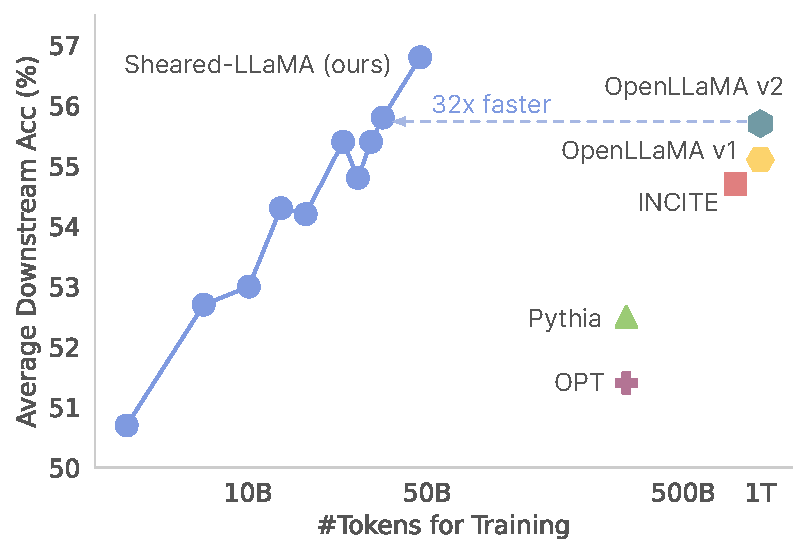
\includegraphics[width=0.92\linewidth]{figures/shearedllama.pdf}
    \caption{Convergence of Sheared LLaMA after structured pruning and continued pre-training,
    compared to other models of similar sizes.
    Plot taken from the original paper ~\citep{xia2024sheared}}
    \label{fig:sheared_llama}
\end{figure}

Some LLM releases have also experimented with pruning to produce smaller 
models from larger ones. For example, the Llama~3.2 1B and 3B models were obtained 
through one-shot structured pruning of Llama~3.1 8B.\footnote{
\url{https://ai.meta.com/blog/llama-3-2-connect-2024-vision-edge-mobile-devices/}}
The pruned models were then trained using knowledge distillation, 
with the logits of Llama~3.1 8B and 70B used as training targets.
Meanwhile, Ministral~3~\citep{liu2026ministral3} uses cascaded pruning and distillation. Starting from Mistral Small~3.1 24B, the authors successively
produce a smaller model at each stage, which is trained using the logits of the original model.
This ``prune--distill--repeat'' procedure is similar to Minitron.

There are some approaches that focus specifically on layer pruning, 
based on the observation that several Transformer layers are redundant \citep{men2024shortgpt, yang2024laco}.
For example, \textbf{ShortGPT}~\citep{men2024shortgpt} measures the contribution 
of each layer using the cosine similarity between its input and output activations. 
The intuition is that an unimportant layer does not substantially modify 
its input representation. Therefore, layers whose input and output activations 
are highly similar can be removed. However, layer pruning generally
incurs a significant performance drop, and the resulting model often requires 
additional training to recover. It is therefore interesting to ask whether, 
in decoder-only LLMs, high layer similarity is a misleading signal for pruning. 
Information flows progressively through the network, and each layer may add only 
a small but important update through the residual connection. 
Although these updates are individually small, they accumulate across dozens 
of layers. Consequently, a high similarity between the input and output of a 
layer does not necessarily mean that the layer is useless. 
Removing several such layers can disrupt this accumulation and degrade 
performance unless a recovery stage is applied. Later evaluations of one-shot 
layer pruning have notably found that it can preserve performance on simple or 
multiple-choice benchmarks while substantially harming open-ended generation 
and long-chain reasoning capabilities~\citep{wang2025fewerlayers,he2026pop}.
\footnote{
    \url{https://www.reddit.com/r/MachineLearning/comments/1bc1638/r_shortgpt_layers_in_large_language_models_are/}
}

\begin{figure}[!ht]
    \centering
    \definecolor{pruningnode}{HTML}{EEE0CC}
    \begin{tikzpicture}[
        neuron/.style={circle, draw=black!75, fill=pruningnode, minimum size=7.5mm, inner sep=0pt},
        kept/.style={black!78, line width=1.05pt},
        flow/.style={-{Latex[length=2.4mm]}, black!70, line width=0.9pt}
    ]
        \begin{scope}
            \node[neuron] (a11) at (0, 0.55) {};
            \node[neuron] (a12) at (0,-0.55) {};
            \node[neuron] (a21) at (1.35, 1.00) {};
            \node[neuron] (a22) at (1.35, 0.00) {};
            \node[neuron] (a23) at (1.35,-1.00) {};
            \node[neuron] (a31) at (2.70, 1.00) {};
            \node[neuron] (a32) at (2.70, 0.00) {};
            \node[neuron] (a33) at (2.70,-1.00) {};
            \node[neuron] (a41) at (4.05, 0.55) {};
            \node[neuron] (a42) at (4.05,-0.55) {};

            \foreach \i in {1,2}
                \foreach \j in {1,2,3}
                    \draw[kept] (a1\i) -- (a2\j);
            \foreach \i in {1,2,3}
                \foreach \j in {1,2,3}
                    \draw[kept] (a2\i) -- (a3\j);
            \foreach \i in {1,2,3}
                \foreach \j in {1,2}
                    \draw[kept] (a3\i) -- (a4\j);

            \node[font=\small\bfseries, anchor=north] at (2.03,-1.55) {Dense network};
        \end{scope}

        \node[font=\footnotesize\bfseries, align=center, anchor=south] at (5.50,0.18) {Structured\\Pruning};
        \draw[flow] (4.85,0) -- (6.15,0);

        \begin{scope}[xshift=7.05cm]
            \node[neuron] (b11) at (0, 0.55) {};
            \node[neuron] (b12) at (0,-0.55) {};
            \node[neuron] (b31) at (2.00, 1.00) {};
            \node[neuron] (b32) at (2.00, 0.00) {};
            \node[neuron] (b33) at (2.00,-1.00) {};
            \node[neuron] (b41) at (4.05, 0.55) {};
            \node[neuron] (b42) at (4.05,-0.55) {};

            \foreach \i in {1,2}
                \foreach \j in {1,2,3}
                    \draw[kept] (b1\i) -- (b3\j);
            \foreach \i in {1,2,3}
                \foreach \j in {1,2}
                    \draw[kept] (b3\i) -- (b4\j);

            \node[font=\small\bfseries, anchor=north] at (2.03,-1.55) {Pruned network};
        \end{scope}
    \end{tikzpicture}
    \caption{Illustration of structured pruning. A full layer is removed, together with all its incoming and outgoing weights.}
    \label{fig:structured}
\end{figure}
\subsection{The best training objective for compression}
We mentioned distillation as a way to compress the capacity of large models into small models,
but there are many other objectives.
What are the best training objectives for compressing LLMs and training
small LLMs? The common training objective for compression is maximum likelihood
estimation, but small LLMs take time to learn. Hence,
it has been proposed to use training objectives that give more \textit{learning signal}
to the small LLM. Let's list them and see how they're used in recent LLM releases.

\subsubsection{Sequence-Level Distillation}
\begin{figure}[!ht]
    \centering
    \definecolor{distillnode}{HTML}{EEE0CC}
    \begin{tikzpicture}[
        scale=1.12,
        every node/.style={transform shape},
        neuron/.style={circle, draw=black!75, fill=distillnode, minimum size=4.4mm, inner sep=0pt},
        link/.style={black!72, line width=0.72pt},
        flow/.style={-{Latex[length=2.4mm]}, black!72, line width=0.9pt},
        module/.style={draw=black!38, rounded corners=1pt, fill=black!2, line width=0.55pt},
        textnode/.style={font=\small}
    ]
        \node[textnode] (x) at (0,1.25) {$x$};
        \node[textnode] (pair) at (0,-1.35) {$(x,\widehat{y})$};

        \draw[module] (1.15,0.25) rectangle (4.45,2.25);
        \draw[module] (1.15,-2.35) rectangle (4.45,-0.35);

        \begin{scope}[xshift=1.60cm, yshift=1.25cm]
            \node[neuron] (t11) at (0, 0.42) {};
            \node[neuron] (t12) at (0,-0.42) {};
            \node[neuron] (t21) at (0.80, 0.65) {};
            \node[neuron] (t22) at (0.80, 0.00) {};
            \node[neuron] (t23) at (0.80,-0.65) {};
            \node[neuron] (t31) at (1.60, 0.65) {};
            \node[neuron] (t32) at (1.60, 0.00) {};
            \node[neuron] (t33) at (1.60,-0.65) {};
            \node[neuron] (t41) at (2.40, 0.42) {};
            \node[neuron] (t42) at (2.40,-0.42) {};
            \foreach \i in {1,2}
                \foreach \j in {1,2,3}
                    \draw[link] (t1\i) -- (t2\j);
            \foreach \i in {1,2,3}
                \foreach \j in {1,2,3}
                    \draw[link] (t2\i) -- (t3\j);
            \foreach \i in {1,2,3}
                \foreach \j in {1,2}
                    \draw[link] (t3\i) -- (t4\j);
            \node[textnode, font=\footnotesize\bfseries, anchor=south] at (1.20,0.95) {Teacher};
        \end{scope}

        \begin{scope}[xshift=2.10cm, yshift=-1.35cm]
            \node[neuron] (s11) at (0, 0.35) {};
            \node[neuron] (s12) at (0,-0.35) {};
            \node[neuron] (s21) at (0.70, 0.55) {};
            \node[neuron] (s22) at (0.70, 0.00) {};
            \node[neuron] (s23) at (0.70,-0.55) {};
            \node[neuron] (s31) at (1.40, 0.35) {};
            \node[neuron] (s32) at (1.40,-0.35) {};
            \foreach \i in {1,2}
                \foreach \j in {1,2,3}
                    \draw[link] (s1\i) -- (s2\j);
            \foreach \i in {1,2,3}
                \foreach \j in {1,2}
                    \draw[link] (s2\i) -- (s3\j);
            \node[textnode, font=\footnotesize\bfseries, anchor=north] at (0.70,-0.95) {Student};
        \end{scope}

        \node[textnode, anchor=west] (sample) at (5.15,1.25) {$\widehat{y} \sim \mathrm{sample}(p_T(\cdot \mid x))$};
        \node[textnode, anchor=west] (loss) at (5.15,-1.35) {$-\log p_S(\widehat{y} \mid x)$};
        \draw[flow] (x) -- (1.15,1.25);
        \draw[flow] (4.45,1.25) -- (sample.west);
        \draw[flow] (pair) -- (1.15,-1.35);
        \draw[flow] (4.45,-1.35) -- (loss.west);
        \draw[flow, rounded corners=3pt] (sample.south) -- (5.15,-0.05) -- (0.55,-0.05) -- (pair.north);
    \end{tikzpicture}
    \caption{Sequence-level distillation. The teacher first generates a complete answer, and the student is then trained on this synthetic sequence.}
    \label{fig:sequence-level-distillation}
\end{figure}

In sequence-level distillation, the small model is trained on texts generated by a larger and more capable model. 
This approach is illustrated in Figure~\ref{fig:sequence-level-distillation}. 
The concept was introduced for machine translation~\citep{kim2016sequence},
where the translations generated by the teacher are used as targets for the student.
In the context of LLMs, this approach became popular with Alpaca~\citep{taori2023alpaca}. Alpaca trained a small LLaMA model on $52$K instruction--response 
pairs generated by the closed-source \texttt{text-davinci-003} model.
However, generating useful synthetic data is not that simple.
The generated answers must be correct, diverse, sufficiently difficult, 
and representative of the capabilities that we want to model. 
The data must also be filtered to remove redundant, low-quality, or unsafe examples. 
This motivated the development of many methods for automating and improving synthetic-data generation.
Orca~\citep{mukherjee2023orca}, for example, uses GPT-4 to generate detailed 
explanations and reasoning traces rather than only short answers. 
Magpie~\citep{xu2024magpie}, on the other hand, generates both instructions and 
responses from a chat LLM without requiring human-written seed instructions. 
Persona Hub~\citep{ge2024persona} improves data diversity by conditioning 
the generation on a large collection of synthetic personas representing 
different backgrounds, occupations, and perspectives.

There has also been a debate about whether a student trained on teacher-generated data 
can outperform its teacher. This appears possible on specific tasks: for example, a much smaller model can outperform a teacher prompted with a few examples
by learning from both its answers and its rationales~\citep{hsieh2023distilling}.
However, this does not mean that the student becomes generally more capable than 
the teacher. Such improvements often require generating multiple candidate 
responses and retaining only the best ones through correctness verification, 
rejection sampling~\citep{yuan2023scaling}, or learned quality and reward functions. 

\subsubsection{Off-policy Knowledge Distillation}
\begin{figure}[!ht]
    \centering
    \definecolor{distillnode}{HTML}{EEE0CC}
    \begin{tikzpicture}[
        scale=1.12,
        every node/.style={transform shape},
        neuron/.style={circle, draw=black!75, fill=distillnode, minimum size=4.4mm, inner sep=0pt},
        link/.style={black!72, line width=0.72pt},
        flow/.style={-{Latex[length=2.4mm]}, black!72, line width=0.9pt},
        match/.style={<->, dashed, black!60, line width=0.8pt},
        module/.style={draw=black!38, rounded corners=1pt, fill=black!2, line width=0.55pt},
        textnode/.style={font=\small}
    ]
        \node[textnode] (dataS) at (0,1.25) {$(x,y)$};
        \node[textnode] (dataT) at (0,-1.25) {$(x,y)$};

        \draw[module] (1.15,0.25) rectangle (4.45,2.25);
        \draw[module] (1.15,-2.25) rectangle (4.45,-0.25);

        \begin{scope}[xshift=2.10cm, yshift=1.25cm]
            \node[neuron] (s11) at (0, 0.35) {};
            \node[neuron] (s12) at (0,-0.35) {};
            \node[neuron] (s21) at (0.70, 0.55) {};
            \node[neuron] (s22) at (0.70, 0.00) {};
            \node[neuron] (s23) at (0.70,-0.55) {};
            \node[neuron] (s31) at (1.40, 0.35) {};
            \node[neuron] (s32) at (1.40,-0.35) {};
            \foreach \i in {1,2}
                \foreach \j in {1,2,3}
                    \draw[link] (s1\i) -- (s2\j);
            \foreach \i in {1,2,3}
                \foreach \j in {1,2}
                    \draw[link] (s2\i) -- (s3\j);
            \node[textnode, font=\footnotesize\bfseries, anchor=south] at (0.70,0.95) {Student};
        \end{scope}

        \begin{scope}[xshift=1.60cm, yshift=-1.25cm]
            \node[neuron] (t11) at (0, 0.42) {};
            \node[neuron] (t12) at (0,-0.42) {};
            \node[neuron] (t21) at (0.80, 0.65) {};
            \node[neuron] (t22) at (0.80, 0.00) {};
            \node[neuron] (t23) at (0.80,-0.65) {};
            \node[neuron] (t31) at (1.60, 0.65) {};
            \node[neuron] (t32) at (1.60, 0.00) {};
            \node[neuron] (t33) at (1.60,-0.65) {};
            \node[neuron] (t41) at (2.40, 0.42) {};
            \node[neuron] (t42) at (2.40,-0.42) {};
            \foreach \i in {1,2}
                \foreach \j in {1,2,3}
                    \draw[link] (t1\i) -- (t2\j);
            \foreach \i in {1,2,3}
                \foreach \j in {1,2,3}
                    \draw[link] (t2\i) -- (t3\j);
            \foreach \i in {1,2,3}
                \foreach \j in {1,2}
                    \draw[link] (t3\i) -- (t4\j);
            \node[textnode, font=\footnotesize\bfseries, anchor=north] at (1.20,-0.95) {Teacher};
        \end{scope}

        \node[textnode] (studentout) at (5.80,1.25) {$p_S(y \mid x)$};
        \node[textnode] (teacherout) at (5.80,-1.25) {$p_T(y \mid x)$};
        \draw[flow] (dataS) -- (1.15,1.25);
        \draw[flow] (4.45,1.25) -- (studentout);
        \draw[flow] (dataT) -- (1.15,-1.25);
        \draw[flow] (4.45,-1.25) -- (teacherout);
        \draw[match] (studentout.south) -- node[right, font=\footnotesize, align=left] {matching\\loss} (teacherout.north);
    \end{tikzpicture}
    \caption{Off-policy distillation. The student and the teacher are evaluated on the same data, and the student distribution is trained to match the teacher distribution.}
    \label{fig:off-policy-distillation}
\end{figure}
In sequence-level distillation, the training signal provided by each token is limited, 
as the student is trained only on the token sampled by the teacher. 
When the synthetic dataset is sufficiently large, the student can nevertheless 
approximate the teacher's probability distribution underlying the generated texts.
A more direct approach to mimicking the teacher's probability distribution 
is \textbf{logit-based knowledge distillation} \citep{distillation}. 
This approach provides a richer 
training signal since the student learns from the teacher's probability 
distribution over the vocabulary at every token position, rather than from only 
the generated token. This process is illustrated in Figure~\ref{fig:off-policy-distillation}.
The data are passed through both the student and the teacher, which produce
a probability distribution over the vocabulary at each token position of 
the gold answer. The student distribution is then compared with the teacher 
distribution on the same data. The loss can be designed in different ways, 
but the most common choice is the \textit{Kullback--Leibler divergence}, 
which encourages the student distribution to match the teacher distribution.

Logit-based distillation has been used to train several open-weight small language 
models. In particular, Gemma~2 and Gemma~3 were trained by distilling larger teacher 
models~\citep{gemmateam2024gemma2,gemmateam2025gemma3technicalreport}. 
And as discussed earlier, knowledge distillation is used as a recovery stage 
after pruning in small model series such as Llama~3.2 and Ministral~3. 
Logit-based knowledge distillation usually outperforms 
training on hard targets alone as the teacher's probability distribution provides 
a richer training signal for every token~\citep{gemmateam2024gemma2,anshumann2025sparselogit}.
For example, the Gemma~2 ablations show that distillation improves both validation 
perplexity and downstream performance across several student sizes. This is
particularly true in low-data regimes~\citep{liu2026understandingkd}.
Hence logit-based distillation seems to be more sample-efficient.

\subsubsection{On-policy Knowledge Distillation}
In sequence-level and off-policy knowledge distillation, the student remains passive: 
it is trained on sequences generated by the teacher or on fixed sequences for which 
the teacher provides feedback. This creates what is known as the \textit{training--inference mismatch}.
During training, the student is trained using \textit{teacher forcing}, meaning that 
the prediction of the $i$-th token is conditioned on the previous tokens from 
the teacher-generated or gold sequence. At inference time, however, 
the student must generate its own tokens and condition subsequent predictions 
on its previous outputs. It may therefore encounter contexts resulting 
from its own mistakes that were never observed during training.
\textbf{On-policy distillation} addresses this mismatch by allowing the student to generate 
sequences during training and using the teacher to provide feedback on the states 
visited by the student. Prior work shows that knowledge distillation
is more effective when the student learns from feedback on its own generated sequences~\citep{agarwal2024onpolicy}.
This method outperforms distillation based only on fixed teacher-generated data.

Figure~\ref{fig:on-policy-distillation} illustrates the process of on-policy distillation. 
The student takes a prompt and generates an answer, which is then evaluated by 
the teacher. More precisely, the teacher provides a probability distribution at each 
token position of the student-generated sequence. The training loss can be designed 
in different ways, using, for example, the forward or reverse Kullback--Leibler 
divergence or the Jensen--Shannon divergence.
On-policy distillation can be understood through the lens of \textbf{reinforcement learning}: 
the student's generations can be seen as actions, while the teacher provides the
reward on those actions. Since the reward is differentiable, training
does not necessarily require policy-gradient algorithms such as REINFORCE.
The student can instead be trained directly by minimizing the token-level divergence 
from the teacher distribution.
Subsequent studies have extended on-policy distillation beyond the compression
of small models and used it as a post-training framework. Recently, 
\textbf{On-Policy Self-Distillation} has emerged as a new post-training 
approach~\citep{zhao2026selfdistilled}. In this setting, the student and 
the teacher are the same model but receive different information. 
The teacher is given \textit{privileged information}, such as the gold answer 
or a verified reasoning trace, whereas the student receives only the original prompt. 
The student generates its own response, and the privileged version of the model 
provides dense token-level feedback on this response. 

\begin{figure}[!ht]
    \centering
    \definecolor{distillnode}{HTML}{EEE0CC}
    \begin{tikzpicture}[
        scale=1.12,
        every node/.style={transform shape},
        neuron/.style={circle, draw=black!75, fill=distillnode, minimum size=4.4mm, inner sep=0pt},
        link/.style={black!72, line width=0.72pt},
        flow/.style={-{Latex[length=2.4mm]}, black!72, line width=0.9pt},
        module/.style={draw=black!38, rounded corners=1pt, fill=black!2, line width=0.55pt},
        textnode/.style={font=\small}
    ]
        \node[textnode] (x) at (0,1.25) {$x$};
        \node[textnode] (pair) at (0,-1.35) {$(x,\widehat{y})$};

        \draw[module] (1.15,0.25) rectangle (4.45,2.25);
        \draw[module] (1.15,-2.35) rectangle (4.45,-0.35);

        \begin{scope}[xshift=2.10cm, yshift=1.25cm]
            \node[neuron] (s11) at (0, 0.35) {};
            \node[neuron] (s12) at (0,-0.35) {};
            \node[neuron] (s21) at (0.70, 0.55) {};
            \node[neuron] (s22) at (0.70, 0.00) {};
            \node[neuron] (s23) at (0.70,-0.55) {};
            \node[neuron] (s31) at (1.40, 0.35) {};
            \node[neuron] (s32) at (1.40,-0.35) {};
            \foreach \i in {1,2}
                \foreach \j in {1,2,3}
                    \draw[link] (s1\i) -- (s2\j);
            \foreach \i in {1,2,3}
                \foreach \j in {1,2}
                    \draw[link] (s2\i) -- (s3\j);
            \node[textnode, font=\footnotesize\bfseries, anchor=south] at (0.70,0.95) {Student};
        \end{scope}

        \begin{scope}[xshift=1.60cm, yshift=-1.35cm]
            \node[neuron] (t11) at (0, 0.42) {};
            \node[neuron] (t12) at (0,-0.42) {};
            \node[neuron] (t21) at (0.80, 0.65) {};
            \node[neuron] (t22) at (0.80, 0.00) {};
            \node[neuron] (t23) at (0.80,-0.65) {};
            \node[neuron] (t31) at (1.60, 0.65) {};
            \node[neuron] (t32) at (1.60, 0.00) {};
            \node[neuron] (t33) at (1.60,-0.65) {};
            \node[neuron] (t41) at (2.40, 0.42) {};
            \node[neuron] (t42) at (2.40,-0.42) {};
            \foreach \i in {1,2}
                \foreach \j in {1,2,3}
                    \draw[link] (t1\i) -- (t2\j);
            \foreach \i in {1,2,3}
                \foreach \j in {1,2,3}
                    \draw[link] (t2\i) -- (t3\j);
            \foreach \i in {1,2,3}
                \foreach \j in {1,2}
                    \draw[link] (t3\i) -- (t4\j);
            \node[textnode, font=\footnotesize\bfseries, anchor=north] at (1.20,-0.95) {Teacher};
        \end{scope}

        \node[textnode, anchor=west] (sample) at (5.15,1.25) {$\widehat{y} \sim \mathrm{sample}(P_{S}(\cdot \mid x))$};
        \node[textnode, anchor=west] (teacherout) at (5.15,-1.35) {$\mathrm{loss}\!\left(p_T(\widehat{y} \mid x) \,\Vert\, p_S(\widehat{y} \mid x)\right)$};
        \draw[flow] (x) -- (1.15,1.25);
        \draw[flow] (4.45,1.25) -- (sample.west);
        \draw[flow] (pair) -- (1.15,-1.35);
        \draw[flow] (4.45,-1.35) -- (teacherout.west);
        \draw[flow, rounded corners=3pt] (sample.south) -- (5.15,-0.05) -- (0.55,-0.05) -- (pair.north);
    \end{tikzpicture}
    \caption{On-policy distillation. The student first samples an output, then the teacher evaluates this student-generated output.}
    \label{fig:on-policy-distillation}
\end{figure}
\section{Our contribution to model compression}
Our contributions address two limitations of post-training compression for
pre-trained Transformers:
\begin{enumerate}
    \item We study low-rank decomposition for compressing pretrained LLMs and
    propose \textbf{Lillama}. The method combines low-rank weight
    approximation with layer-wise distillation, and it explicitly addresses the
    \textbf{training--inference mismatch} discussed so far by making the distillation more
    \textbf{on-policy}: each student layer is trained on activations produced by
    preceding student layers, rather than on teacher-only features. 
    Compared with unstructured or semi-structured pruning methods such as
    \textbf{SparseGPT}~\citep{frantar2023sparsegpt} and
    \textbf{Wanda}~\citep{sun2024wanda}, which rely on sparse weight formats
    and specialized kernels to achieve speedup, Lillama shrinks the parameters
    of the LLM and naturally saves computation. It also differs
    from structured pruning pipelines such as
    \textbf{Sheared LLaMA}~\citep{xia2024sheared} and
    \textbf{Minitron}~\citep{muralidharan2024compact,sreenivas2024minitron},
    which require more expensive retraining stages after pruning. In contrast,
    Lillama keeps the compression local and one-shot: it compresses only
    selected layers, initializes them with SVD, and distills them with a small
    calibration set while preserving the dense execution path and the original
    model structure.

    \item Post-training compression often leaves the LM head untouched because
    compressing it can distort the output probability distribution and force a
    costly recovery stage. We propose \textbf{BaldWhisper}, showing that
    low-rank compression of the head together with feature distillation offers a
    good speed--accuracy trade-off despite the \textbf{softmax bottleneck}.
    We also study \textbf{layer merging} as an alternative to layer pruning,
    reducing decoder depth to lower self-attention and cross-attention costs
    during autoregressive decoding, which is \textbf{memory-bound}. This
    places our work in the same compression regime as low-rank approximations,
    distillation, and structured pruning, but targets a part of the model that
    is commonly left untouched in standard post-training compression pipelines.
\end{enumerate}

\section{Activation Sparsity}
While post-training compression of LLMs has proved to be an effective approach
to create small LLMs, larger LLMs nevertheless remain more performant.
They generalize better, contain more knowledge, and are much better at
in-context learning. However, as discussed, they are also more costly to train
and to serve for inference. Can we get some of the benefits of large models,
but at a lower training and inference cost? Sparse activation is one answer
to this question. The model dynamically selects which parameters should be used 
for the current input token. The selected parameters are called \textbf{active parameters}, 
while the others remain inactive for this specific input.
When associated with efficient GPU kernels, sparsity reduces the activation memory,
so it gives more room for larger batches and hence higher training and inference \textbf{throughput}. 
It can also accelerate the end-to-end decoding speed.

Sparse activations make it possible to partly decouple model size from
computation, and provide new scaling axes compared to dense models:

\begin{enumerate}
    \item \textbf{Sparsity scaling axis}: keeping the number of active parameters per input fixed, 
    while increasing the total number of model parameters.
    \item \textbf{Computation scaling axis}: keeping the total number of parameters fixed, 
    while increasing the computation by activating more parameters per input.
    \item \textbf{Granularity scaling axis}: increasing the number of experts while keeping 
    the number of activated parameters and the model parameters fixed.
\end{enumerate}
Training sparse models is difficult because the process of selecting which
parameters to activate is often discrete and therefore not directly
differentiable. However, the know-how has evolved a lot, especially for
sparse mixtures of experts, which are now the most successful class of sparse models at
scale. We will present different classes of sparse models, their pros and cons,
and particularly the optimization tricks that make their training possible.

\subsection{Sparse Mixture of Experts (MoE)}

\begin{figure}[!ht]
    \centering
    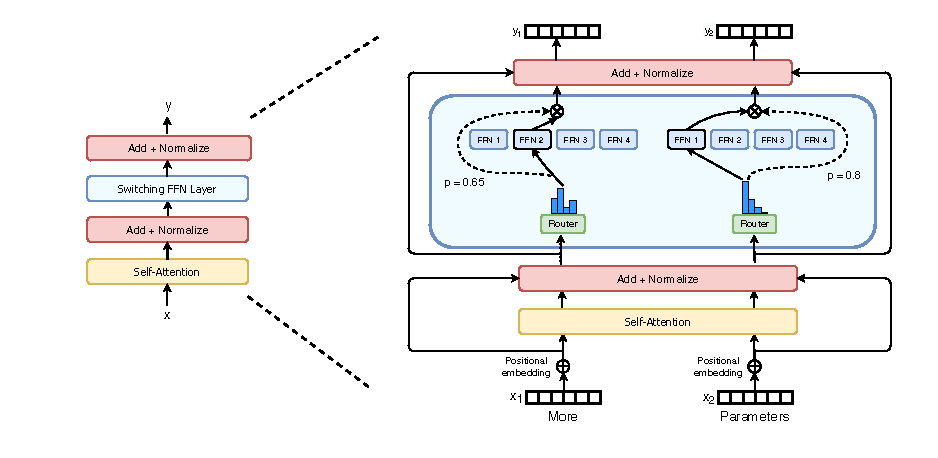
\includegraphics[width=1.0\linewidth]{figures/switch_transformer_figure2.pdf}
    \caption{Switch Transformer encoder block, where the dense feed-forward layer
    is replaced by a sparse Switch FFN layer. Figure adapted from
    \citep{switch}.}
    \label{fig:switch-transformer-block}
\end{figure}

\subsubsection{The MoE layer}
In a sparse MoE, the weight matrix $\mathbf{W}$ is split into $e$ submatrices called experts,
$\mathbf{W}_1, \ldots, \mathbf{W}_e$. The model is trained to decide which
experts are useful for the current input $\mathbf{x}$, and evaluates only these
experts. Thus, the model can contain many parameters, while each token only
activates a small fraction of them. The selection of the experts is performed 
by a router network $R_\theta$ and
the top-$k$ operator. More formally, let $\mathbf{x} \in \mathbb{R}^{d_1}$ be
the input, and let each expert $\mathbf{W}_j \in \mathbb{R}^{d_1 \times d_e}$.
The router produces one logit, or score, per expert,
$\mathbf{r}=R_\theta(\mathbf{x}) \in \mathbb{R}^{e}$. The top-$k$ operator is
first applied to these router logits to select the subset of active experts,
$S = \{j \mid r_j \in \mathrm{TopK}(\mathbf{r}, k)\}$. Then, the routing
weights are computed with a softmax only over these selected experts. Thus, for
each selected expert $j \in S$, we have
$g_j = \exp(r_j) / \sum_{\ell \in S} \exp(r_\ell)$.
The output of a sparse MoE layer is then the weighted sum of these selected
experts:
\begin{equation}
    o = \mathrm{MoE}(\mathbf{x})
    =
    \sum_{j \in S}
    g_j \mathbf{W}_j^\top \mathbf{x}.
\end{equation}
The output of the MoE layer is then projected back to the model dimension $d_{model}$.

\subsubsection{The nice scaling properties of MoEs}
MoEs give a way to increase the capacity of the model without increasing 
the computation by the same factor. Switch Transformer~\citep{switch} shows that at a FLOP-matched
budget, increasing the number of experts improves the overall performance.
This means increasing the model parameters while keeping the same number of
activated parameters is beneficial. Figure~\ref{fig:switch} illustrates this. 
On the left plot, we can see that keeping the number of activated parameters fixed,
while increasing the number of experts, leads to substantial improvements. However,
it doesn't seem linear, and at some point increasing the number of parameters
without increasing the number of activated parameters stops being beneficial.
And since bigger models converge faster, large MoEs also accelerate training
as shown by the right plot.

\begin{figure}[!ht]
    \centering
    \subfloat[Validation loss as the number of parameters increases.]{
        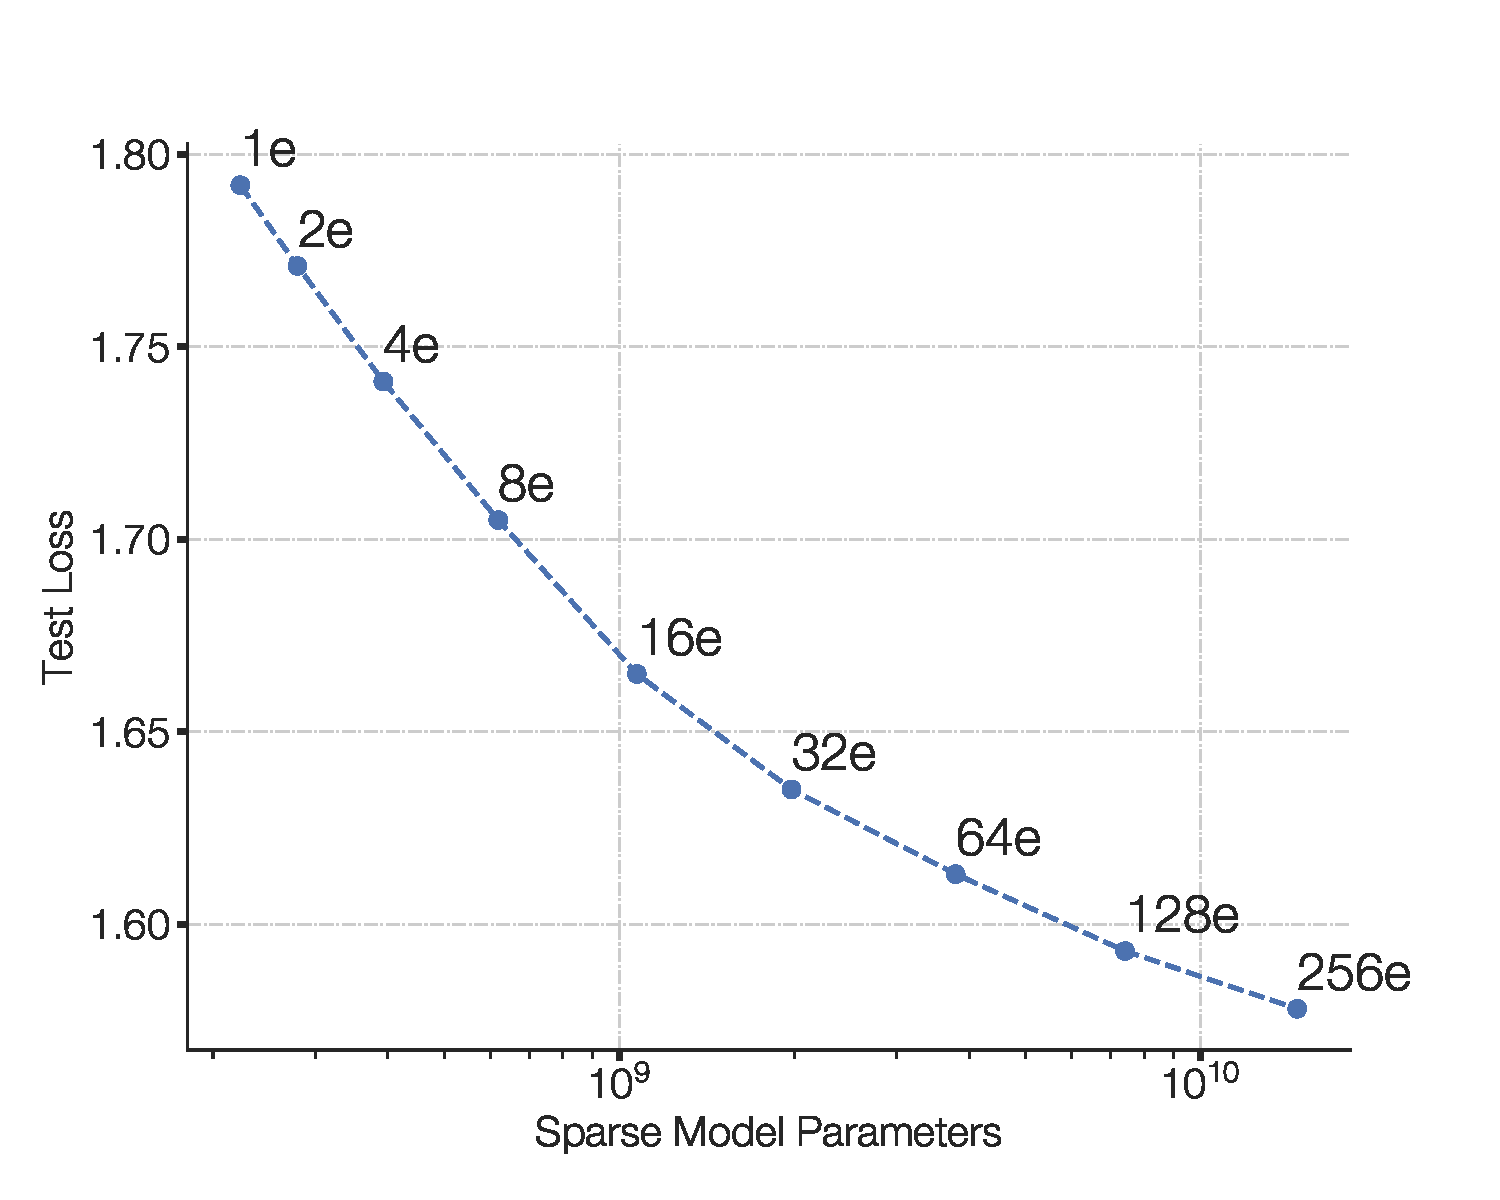
\includegraphics[width=0.48\linewidth]{figures/loss_vs_log_params.pdf}
    }
    \hfill
    \subfloat[Negative log-perplexity during training.]{
        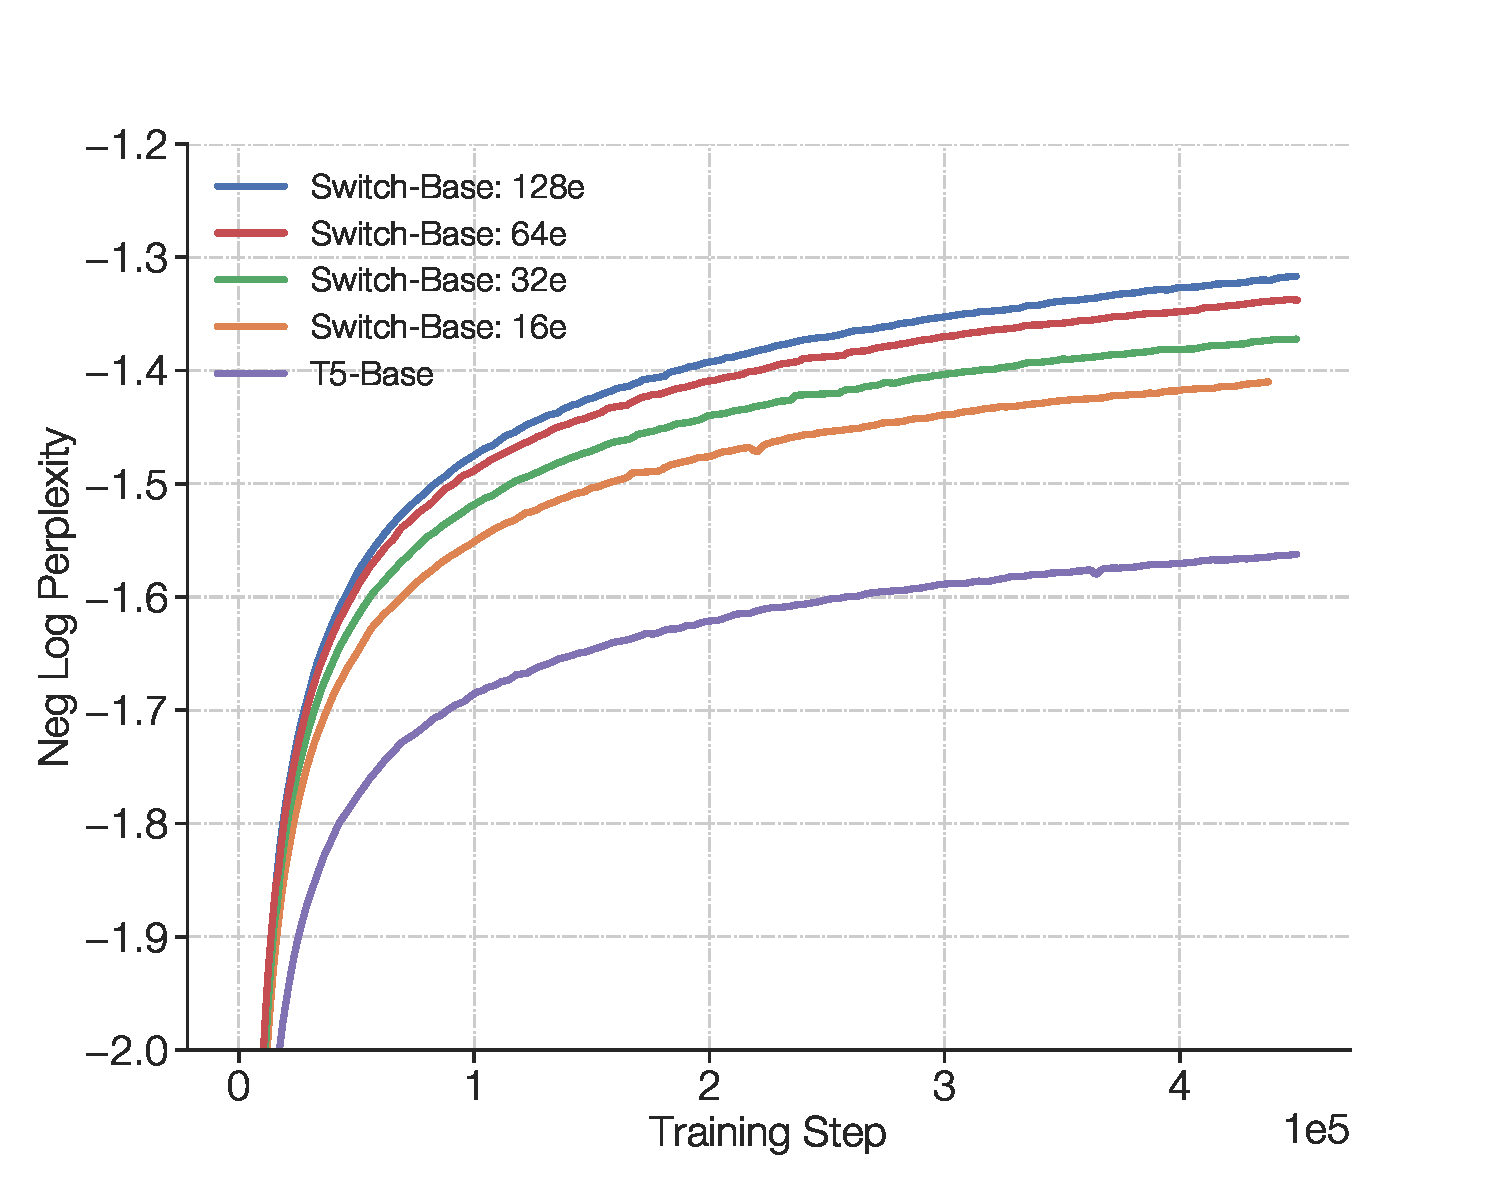
\includegraphics[width=0.48\linewidth]{figures/perp_vs_step.pdf}
    }
    \caption{Scaling properties of Switch Transformer. Increasing the number of experts improves performance and sample efficiency at equal computational budget. Figure from \citep{switch}.}
    \label{fig:switch}
\end{figure}
Sparsity has been pushed much further in recent sparse MoEs. The DeepSeek
series particularly pushed fine-grained experts and very sparse activation.
DeepSeek-V3 uses $256$ routed experts and activates only $8$ of them for each
token, which represents approximately $97\%$ sparsity~\citep{deepseekai2024deepseekv3}.
DeepSeek-V4-Pro pushes this even further: it has $384$ routed experts and activates only $6$ per
token, so more than $98\%$ of the routed experts are inactive at each
step~\citep{deepseekai2026deepseekv4}. Since MoEs decouple parameter
scaling from computation, recent models therefore scale to
multi-trillion-parameter sparse MoEs, such as Kimi-K3 with $2.8$T parameters
and $104$B active parameters~\citep{moonshotai2026kimik3}, or Qwen3.8-Max with
$2.4$T parameters and $95$B active parameters~\citep{qwen2026qwen38}.

Beyond the scaling axis between active parameters and total parameters, MoEs
also introduce another important axis: \textbf{granularity}, namely how many
experts are available. This is different from sparsity. For example,
with $50\%$ sparsity, one can activate $1$ expert out of $2$, or $1024$ experts
out of $2048$. Both designs activate the same fraction of experts, and can have
the same total number of parameters, but the second design is much more
fine-grained. It gives the router many more possible combinations of experts.
In \citep{krajewski2024scaling}, the authors study this effect while keeping the
model size and the number of training tokens fixed. 
As illustrated in Figure~\ref{fig:fine-grained-moe-granularity}, 
their main result is that increasing granularity usually improves loss, 
probably because it gives the router more flexibility to combine experts.
The model can represent a more precise mixture of skills. 
\begin{figure}[!ht]
    \centering
    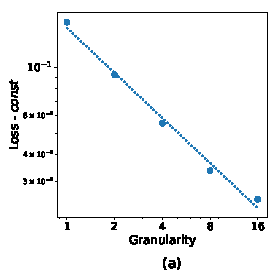
\includegraphics[width=0.9\linewidth]{figures/fine_grained_moe_granularity_figure3a.pdf}
    \caption{Effect of MoE granularity on loss for fixed model size and number of training tokens. Figure adapted from \citep{krajewski2024scaling}.}
    \label{fig:fine-grained-moe-granularity}
\end{figure}

\subsubsection{Stabilizing MoEs}
Scaling large, sparse, and fine-grained MoEs produces strong, efficient models,
but also makes training challenging. This is true in terms of infrastructure:
more experts create communication overhead between nodes and GPUs, as well as
uneven GPU memory use when some experts are used more than others.
It is also true in terms of optimization dynamics: TopK-based routing
is not differentiable, which complicates optimization and requires
many tricks to stabilize training.

\paragraph{Load Balancing.} The router must learn to distribute tokens across experts.
If most tokens are routed to the same few experts, these experts become
overloaded, while the other experts receive almost no training. Their hosting GPUs
also receive more work than the others, which unbalances the GPU cluster.
Switch Transformer avoids this by adding what is called a \textbf{load balancing}
auxiliary loss, a loss added to the language modeling loss to encourage more
uniform token routing at the batch level. There are several load balancing
approaches. DeepSeek-V2 uses three types of auxiliary load balancing
losses~\citep{deepseekai2024deepseekv2}:
\begin{itemize}
    \item \textit{Expert-level load balance}: encourages tokens to be distributed
    more uniformly across experts to avoid router collapse, 
    so that no expert is overloaded and no expert remains undertrained.
    \item \textit{Device-level load balance}: encourages the total expert load to
    be balanced across devices, since groups of experts are stored on different
    GPUs or nodes.
    \item \textit{Communication balance}: avoids sending too many tokens to the same
    device during routing.
\end{itemize}
These are auxiliary losses added to the main task loss, which is the language
modeling loss. This can hurt the optimization of the main language modeling
task, because the model is partly optimized to satisfy a routing constraint
instead of only predicting the next token. For this reason, recent large sparse
MoEs often move toward \textbf{auxiliary-loss-free load balancing}, where
balancing is not directly added to the training loss. 
DeepSeek-V3 uses a bias-based auxiliary-loss-free balancing strategy
\citep{deepseekai2024deepseekv3,wang2024auxiliarylossfree}. A bias
$\mathbf{b} \in \mathbb{R}^{e}$ is added to the router scores for the
top-$k$ selection. The final routing weights are still computed from the
original router scores, without this bias. During training, the expert load is
monitored at each step: if an expert is overloaded, its bias is decreased by a
small constant; if it is underloaded, its bias is increased. Hence the router is
progressively pushed toward balanced expert usage, but without creating
additional gradients for a balancing constraint.
Kimi-K3 uses a related but more direct approach called \textbf{Quantile
Balancing}~\citep{moonshotai2026kimik3}, which computes an expert-specific
threshold from the quantiles of the router scores such that overused experts
receive a harder threshold and underused experts receive an easier one.

\paragraph{Waking the Dead.} Even with load balancing constraints,
large-scale fine-grained sparse MoEs can lead to instabilities. And some of
them are silent. In Step 3.5 Flash~\citep{stepfun2026step35flash}, 
the authors report what they call \textbf{dead experts}, 
in comparison to the \textbf{dead neurons} phenomenon
observed in ReLU-like activations. An expert is dead when it
receives almost no useful training signal. In the simplest case, the router does
not dispatch tokens to this expert for a long period, so the expert receives
almost no gradient. But the Step 3.5 Flash report also shows a more subtle case:
the router statistics can look healthy, while the expert itself is collapsing.
The expert is selected, but its activations are not meaningful, and its parameter norms
become stagnant or decay.
A recent blog post\footnote{
    \url{https://alltoall.notion.site/save-lower-layer-moe-experts-llal}
} on ultra-sparse MoEs makes a similar observation: lower-layer
experts can silently collapse even when training loss, validation loss and load
balancing metrics look normal~\citep{jin2026llalmoe}.
Their proposed solution, \textbf{LM Loss as Auxiliary Loss} (LLAL), is to
temporarily compute the language modeling loss using the output of the collapsing MoE layers, 
so they are "forced" to become useful.

\subsubsection{Are "experts" really experts?}
There is a debate about whether experts can specialize in particular
domains. So far, there is no clear evidence of \textbf{expert specialization} in MoE LLMs,
at least not in the intuitive sense of "specialization" on domains such as code,
math, literature, etc. Mixtral is among the first open sparse MoE LLMs to study
this question directly~\citep{jiang_mixtral_2024}. 
The authors measure how often each expert is selected on different subsets of
The Pile, such as ArXiv, GitHub, PubMed, PhilPapers or Wikipedia. If experts
were domain experts, we would expect some experts to be often selected
for some domains. But this is not what happens. As shown in
Figure~\ref{fig:mixtral-expert-selection-domains}, the routing across different domains is
mostly uniform. However, they find that neighboring tokens in the sequence
tend to be assigned to the same experts.

\begin{figure}[!ht]
    \centering
    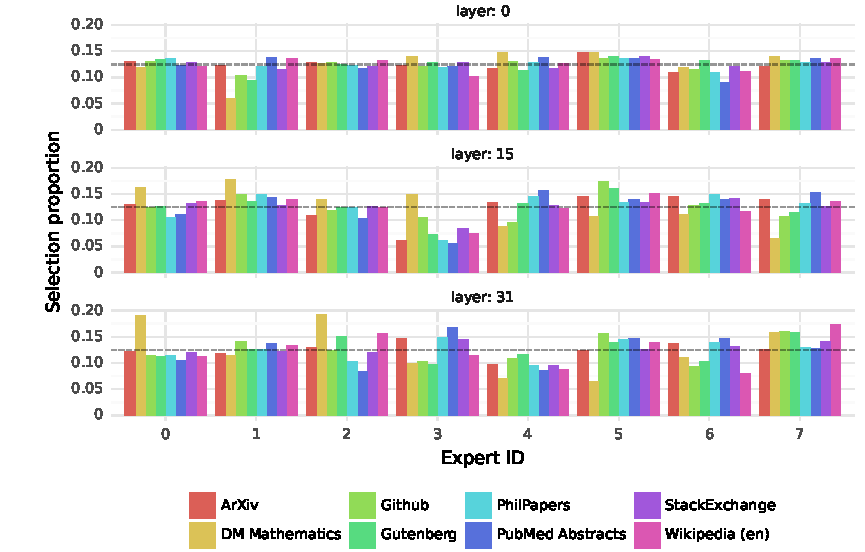
\includegraphics[width=1.0\linewidth]{figures/mixtral_expert_selection_domains.pdf}
    \caption{Expert selection proportions in Mixtral across domains and layers.
    The dashed line corresponds to uniform routing over the eight experts.
    Figure adapted from \citep{jiang_mixtral_2024}.}
    \label{fig:mixtral-expert-selection-domains}
\end{figure}

Expert specialization can be more salient on surface forms, such as
scripts and language families. NLLB-200, which is a sequence-to-sequence MoE
machine translation model, studies this by measuring the similarity between
languages according to their gating decisions~\citep{nllbteam2022nolanguageleftbehind}.
As shown in Figure~\ref{fig:nllb-moe-language-similarity}, the late decoder MoE
layer clearly separates languages: languages from the same family tend to select
similar experts. The early encoder layer also shows some language-expert
specialization. This suggests that expert specialization exists, but it is
not necessarily a clean semantic specialization. This finding is also
supported by observations in OLMoE, where the authors observe a strong vocabulary-level
specialization of experts~\citep{muennighoff2025olmoe}. Some experts specialize
in scripts or alphabets, others in punctuation, religious terms, dates, places,
family words, or technical tokens. In other words, experts can specialize, but
not always in high-level domains such as math or code. The specialization can
also reflect scripts, language families, token forms, and vary depending on the
position of the MoE layer.

\begin{figure}[!ht]
    \centering
    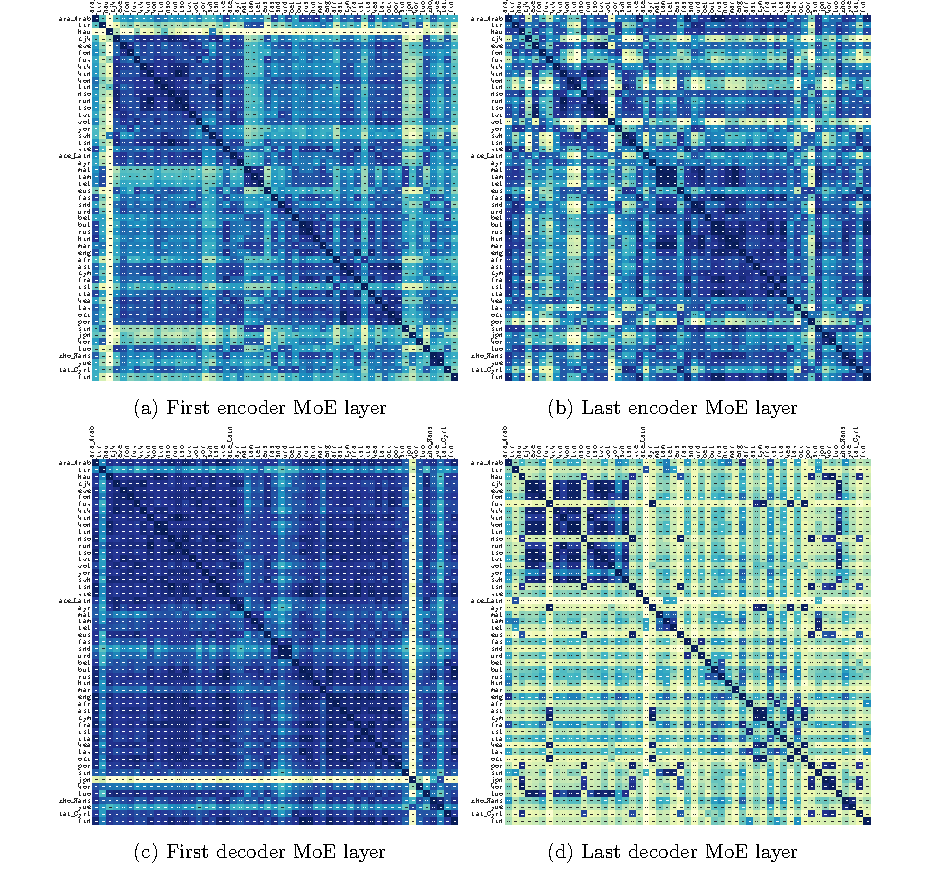
\includegraphics[width=1.0\linewidth]{figures/nllb_moe_language_similarity_figure20.pdf}
    \caption{Cosine similarity between languages based on expert-choice patterns
    in NLLB-200. Figure adapted from \citep{nllbteam2022nolanguageleftbehind}.}
    \label{fig:nllb-moe-language-similarity}
\end{figure}

\begin{table}[!ht]
    \centering
    \footnotesize
    \setlength{\tabcolsep}{2.2pt}
    \renewcommand{\arraystretch}{0.92}
    \newcommand{\olmoetok}[1]{\colorbox{insightback}{\strut #1}}
    \newcommand{\olmoeglyph}[1]{\includegraphics[height=.78em]{figures/olmoe_unicode/#1}}
    \resizebox{\linewidth}{!}{%
    \begin{tabular}{p{1.4cm} p{6cm} p{6cm}}
        \toprule
        \textbf{Expert ID} & \textbf{Input token IDs} & \textbf{Token IDs generated while the expert is active} \\
        \midrule
        27 &
        \olmoetok{\olmoeglyph{copyright}} (100\%) \olmoetok{\olmoeglyph{latin_l}} (100\%) \olmoetok{$^{3}$} (100\%)
        \olmoetok{\olmoeglyph{latin_i}} (100\%) \olmoetok{\olmoeglyph{jarai_i}} (100\%)
        \olmoetok{\olmoeglyph{devanagari_virama}} (100\%) \olmoetok{\olmoeglyph{devanagari_e}} (100\%)
        \olmoetok{\olmoeglyph{devanagari_ka}} (100\%) \olmoetok{\olmoeglyph{cyrillic_sha}} (100\%)
        \olmoetok{\olmoeglyph{cyrillic_in}} (100\%) \olmoetok{\olmoeglyph{cyrillic_a}} (100\%) &
        \olmoetok{\olmoeglyph{slovak_l}} (100\%) \S{} (100\%)
        \olmoetok{\olmoeglyph{copyright}} (100\%) \olmoeglyph{persian_j} (100\%)
        \olmoetok{\olmoeglyph{dutch_ij}} (100\%) \olmoetok{\olmoeglyph{chinese_dot}} (100\%)
        \olmoetok{\olmoeglyph{japanese_no}} (100\%) \olmoetok{\olmoeglyph{devanagari_ra}} (100\%)
        \olmoetok{\olmoeglyph{devanagari_ka}} (100\%) \olmoetok{\olmoeglyph{devanagari_virama}} (100\%)
        \olmoetok{\olmoeglyph{devanagari_la}} (100\%) \\
        \midrule
        58 &
        \olmoetok{(``} (100\%) \olmoetok{("} (100\%) \olmoetok{`} (94\%)
        \olmoetok{'} (92\%) \olmoetok{``} (92\%) \olmoetok{(} (92\%)
        \olmoetok{"} (90\%) \olmoetok{'} (89\%) \olmoetok{``} (88\%)
        \olmoetok{\$} (87\%) \olmoetok{[} (87\%) \olmoetok{pound} (86\%) &
        \olmoetok{such} (100\%) \olmoetok{486} (100\%) \olmoetok{see} (95\%)
        \olmoetok{which} (91\%) \olmoetok{driving} (91\%) \olmoetok{UK} (90\%)
        \olmoetok{who} (88\%) \olmoetok{including} (88\%) \olmoetok{normal} (88\%) \\
        \midrule
        7 &
        \olmoetok{Him} (100\%) \olmoetok{inde} (100\%) \olmoetok{Jesus} (98\%)
        \olmoetok{God} (90\%) \olmoetok{pray} (81\%) \olmoetok{Holy} (80\%)
        \olmoetok{Quran} (80\%) \olmoetok{God} (77\%) \olmoetok{Lord} (76\%)
        \olmoetok{glory} (75\%) \olmoetok{Spirit} (66\%) \olmoetok{Christ} (65\%) &
        \olmoetok{rella} (100\%) \olmoetok{Him} (94\%) \olmoetok{sin} (90\%)
        \olmoetok{prince} (80\%) \olmoetok{glory} (72\%) \olmoetok{Jesus} (69\%)
        \olmoetok{Lord} (68\%) \olmoetok{Christ} (65\%) \olmoetok{Spirit} (55\%)
        \olmoetok{Holy} (53\%) \olmoetok{God} (50\%) \olmoetok{Prayer} (50\%) \\
        \midrule
        37 &
        \olmoetok{Sunday} (100\%) \olmoetok{Tuesday} (100\%) \olmoetok{Thursday} (100\%)
        \olmoetok{Olympic} (100\%) \olmoetok{Christmas} (100\%) \olmoetok{rugby} (100\%)
        \olmoetok{Championship} (100\%) \olmoetok{weekends} (100\%) &
        \olmoetok{days} (91\%) \olmoetok{anniversary} (90\%) \olmoetok{month} (88\%)
        \olmoetok{week} (84\%) \olmoetok{mpi} (83\%) \olmoetok{semester} (81\%)
        \olmoetok{mand} (80\%) \olmoetok{Olympics} (78\%) \olmoetok{cent} (76\%)
        \olmoetok{season} (76\%) \olmoetok{perm} (75\%) \\
        \midrule
        3 &
        \olmoetok{grandmother} (92\%) \olmoetok{brother} (91\%) \olmoetok{Daisy} (83\%)
        \olmoetok{daughter} (78\%) \olmoetok{mum} (75\%) \olmoetok{father} (72\%)
        \olmoetok{wife} (70\%) \olmoetok{husband} (70\%) \olmoetok{lady} (63\%)
        \olmoetok{dad} (62\%) \olmoetok{boy} (61\%) &
        \olmoetok{hood} (36\%) \olmoetok{mother} (35\%) \olmoetok{inde} (31\%)
        \olmoetok{boy} (29\%) \olmoetok{girl} (28\%) \olmoetok{married} (27\%)
        \olmoetok{tri} (21\%) \olmoetok{Gab} (20\%) \olmoetok{died} (18\%)
        \olmoetok{taught} (14\%) \olmoetok{lived} (13\%) \olmoetok{knew} (10\%) \\
        \bottomrule
    \end{tabular}%
    }
    \caption{Vocabulary specialization in the seventh layer of OLMoE-1B-7B.
    Table adapted from \citep{muennighoff2025olmoe}.}
    \label{tab:olmoe-vocabulary-specialization}
\end{table}

\subsubsection{On the non-adaptivity of TopK}
Liam Fedus, first author of Switch Transformer together with Noam Shazeer,
reports that Shazeer once intuited:
``Parameters is knowledge, FLOPs is intelligence.''\footnote{
    \url{https://x.com/LiamFedus/status/2090363702042304847?s=20}
}
In this view, increasing the number of experts while keeping the number of
activated parameters fixed mainly increases the model's knowledge capacity.
It does not increase the computation spent on each token. So the gain should
be weaker on tasks that require more computation rather than more memorized
knowledge. The natural next step is therefore to make sparse LLMs adaptive:
use more experts when the token or the task is hard, and use fewer experts
when it is not.

This intuition is now widely shared in the field, and many works propose ways
to make MoE routing compute-adaptive\footnote{
    See this blog post for an overview of the approaches
    \url{https://huggingface.co/blog/Spico/dynamic-routing}
}. One proposed routing strategy is inspired by
TopP decoding~\citep{huang2024hardertasksneedexperts}. Unlike TopK, TopP does not activate a fixed number of experts.
It sorts the router probabilities and keeps the smallest set of experts whose
cumulative probability is above a threshold $p$. When the router is confident,
only a few experts are used. When the distribution is flatter, more experts are
activated.

Another approach is to replace the hard TopK operation with a continuous ReLU
router \citep{wang2025remoefullydifferentiablemixtureofexperts}. In that case,
experts with positive router scores are active, and sparsity is encouraged during
training by regularizing these scores. The number of active experts is
therefore not fixed, but emerges from the input and from training.

The most commonly used adaptive sparse MoE approach at scale is probably the
\textbf{zero-computation expert}. This method adds identity experts that
let the input pass through without computation.
This approach is used, for example, in LongCat-Flash
\citep{meituanlongcatteam2025longcatflashtechnicalreport}, 
where they encourage a sparsity budget by selecting $K$ experts among both
FFN experts and zero-computation experts. The constraint is 
on the average number of real FFN experts selected by the router. 
The auxiliary-free bias is then adjusted
during training to push this average toward the target budget. In practice, the
model still routes each token to $K$ experts, 
but some of these experts cost almost nothing, so the effective compute 
can change from token to token.

\begin{figure}[tb]
    \centering
    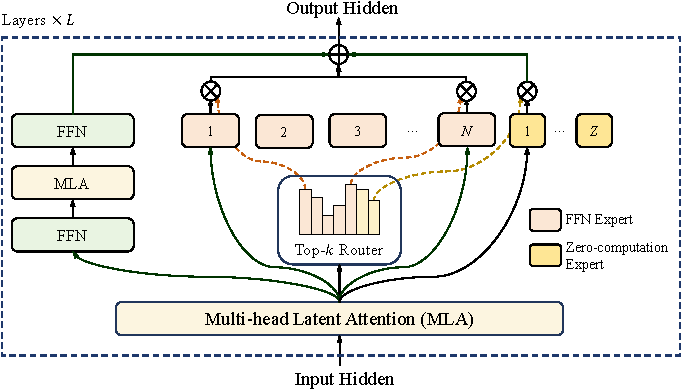
\includegraphics[width=1.0\linewidth]{figures/longcat_flash_architecture.pdf}
    \caption{LongCat-Flash architecture with zero-computation experts.
    The router still selects $K$ experts, but some selected experts are
    identity paths, which makes the effective compute adaptive.
    Figure from \citep{meituanlongcatteam2025longcatflashtechnicalreport}.}
    \label{fig:longcat-flash-architecture}
\end{figure}

\subsection{Sparse Memory Layers}
We discussed \textbf{granularity}, and have shown that increasing the number
of experts, while keeping both the total model size and the number of activated
parameters fixed, can greatly improve performance
(see Figure \ref{fig:fine-grained-moe-granularity}). The extreme case of granularity
would be at the neuron level: each column of the MLP weights can be seen as a
small expert, and only a few of them are activated for a given token. Doing so
turns the dense MLP into a \textbf{sparse memory layer}. 
We mentioned earlier, in the introduction, that the MLP in a Transformer can be
seen as a key-value memory, and that several empirical results support this
view. If this is true, then we can also argue that not all key-value entries are
needed for every input token. Some entries should be useful for one token, and
irrelevant for another one. The natural idea is therefore to make the MLP sparse.
While this approach is less common than MoE to build sparse Transformers, it has
some interesting advantages.

The idea of augmenting neural networks with a large memory is not new \citep{weston2015memorynetworks},
but it has been developed into an efficient approach
that can scale to modern LLMs~\citep{lample2019largememorylayersproduct}.

\begin{figure}[tb]
    \centering
    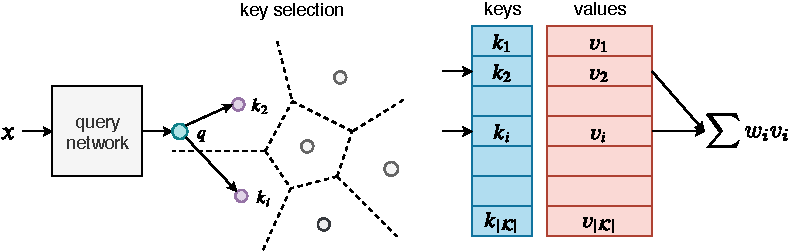
\includegraphics[width=1.0\linewidth]{figures/key_value_memory_layer.pdf}
    \caption{Overview of a key-value memory layer. The input is projected into
    a query, compared to the memory keys, and only the values associated with
    the selected keys are used for computation. Figure from \citep{lample2019largememorylayersproduct}.}
    \label{fig:key-value-memory-layer}
\end{figure}

Following the notation used in prior work~\citep{lample2019largememorylayersproduct},
a memory layer is a function $m:\mathbb{R}^{d}\to\mathbb{R}^{n}$. Given an input
$x \in \mathbb{R}^{d}$, a query network produces a query vector
$q(x)\in\mathbb{R}^{d_q}$. This query is compared to a set of trainable keys
$\mathcal{K}=\{k_1,\ldots,k_{|\mathcal{K}|}\}$, with
$k_i\in\mathbb{R}^{d_q}$, and each key is associated with a trainable value
$v_i\in\mathbb{R}^{n}$.
The memory does not read all values. It first selects the $k$ keys whose inner
product with the query is the largest:
\begin{equation}
    \mathcal{I}
    = \mathcal{T}_{k}\left(\left(q(x)^\top k_i\right)_{i=1}^{|\mathcal{K}|}\right),
\end{equation}
where $\mathcal{T}_{k}$ denotes the TopK operator. Then, the scores of the
selected keys are normalized:
\begin{equation}
    w = \mathrm{Softmax}\left(\left(q(x)^\top k_i\right)_{i\in\mathcal{I}}\right),
\end{equation}
and the output of the memory layer is the weighted sum of the selected values:
\begin{equation}
    m(x) = \sum_{i\in\mathcal{I}} w_i v_i.
\end{equation}
The query decides which memory entries are relevant for the input,
and only these entries are read and updated.
The issue is that, in this simple version, selecting the TopK keys requires
comparing the query to all keys. This is extremely costly for modern
LLM scaling. And the promise of Sparse Memory Layers is to scale the
memory database to millions or even billions of entries, which
is impossible to achieve in the current form.
There are some efficient alternatives to this, which we will
present next.

\subsubsection{Scaling Memory Layers}
\paragraph{Product-Key Memory}
Product-Key Memory (PKM) \citep{lample2019largememorylayersproduct} 
makes key search scalable by using a product structure.
Instead of searching through one huge set of keys, PKM trains two smaller sets of keys,
$\mathcal{K}_1$ and $\mathcal{K}_2$. A full key is not stored directly. It is
formed by combining one key from the first set and one key from the second set.
If $|\mathcal{K}_1|=|\mathcal{K}_2|=m$, this gives $m^2$ possible memory
entries while storing only $2m$ key vectors. The query is also split in two,
$q(x) = [q_1(x), q_2(x)]$, and the score of a composed key is computed as
$q_1(x)^\top k_i^1 + q_2(x)^\top k_j^2$. So the system first
finds the best keys in $\mathcal{K}_1$ and the best keys in $\mathcal{K}_2$,
then combines these candidates to recover the best pairs. Each selected pair
points to a value vector, and the output is still the weighted sum of the
selected values, exactly as in the ordinary memory layer.
In a standard memory, each memory entry has its own explicit key, 
and the query must be compared to all keys. The cost of retrieval therefore grows 
directly with the number of memory entries. 
In PKM, the memory is still large, but its keys are factorized.
The model first searches in two small key tables, which is cheap, and only then
forms a small set of candidate pairs. The expensive comparison with all possible
composed keys is avoided.

\paragraph{Ultra Sparse Memory}
Ultra-Sparse Memory, or UltraMem, is a modern attempt to make PKM
actually competitive at LLM scale \citep{huang2025ultrasparsememorynetwork}
by improving several practical weak points of PKM.
First, they increase the diversity of the values that can be activated. 
They achieve this by halving the value dimension $D_v$, which allows them to double the
number of values while keeping the number of activated value parameters
fixed. The model can access more, smaller values and compose a richer output.
Second, they observe that PKM is \textbf{memory-bound} during training. A very large
sparse memory layer requires few FLOPs, but it can be expensive in memory access and
communication. By splitting the huge memory into several smaller memories
placed across the network, UltraMem avoids concentrating all memory access 
in a single blocking operation. The memory lookups become smaller and more distributed, 
making it easier to overlap them with the standard Transformer computation during training.
Finally, they revisit the product-key decomposition itself with a richer approach
for the query-key retrieval.

\paragraph{Mixture of Million Experts}
Another direction is to keep the product-key retrieval mechanism, but remove the
key-value memory interpretation. This is the idea of PEER (Parameter Efficient
Expert Retrieval)~\citep{he2024mixturemillionexperts}. Conceptually,
PEER is similar to a very fine-grained MoE. Instead of a simple linear layer,
the router uses product keys to retrieve experts efficiently, as in PKM, 
but each retrieved item is not a value vector stored in memory but a tiny MLP expert.
Each expert is reduced to the smallest possible MLP: one up
projection vector, one non-linearity, and one down projection vector. So an
expert is a single hidden neuron. The layer retrieves only a few of these
tiny experts and sums their outputs with router weights.
The difference with PKM is therefore what is retrieved. PKM retrieves
values from a key-value memory whereas PEER retrieves tiny experts. This makes the
layer more naturally connected to MoE scaling and granularity: instead of having
a few large experts, PEER pushes the idea to the extreme by using a large
number of very small experts, while product-key retrieval keeps the routing cost
cheap. Listing~\ref{lst:peer-forward} gives the intuition of the forward pass,
following the pseudocode in the original paper~\citep{he2024mixturemillionexperts}.

\begin{lstlisting}[
  float=tb,
  language=Python,
  frame=tb,
  backgroundcolor=\color{black!3},
  rulecolor=\color{black!25},
  keywordstyle=\color{magenta!80!black}\bfseries,
  commentstyle=\color{green!55!black}\ttfamily,
  stringstyle=\color{violet!80!black},
  identifierstyle=\color{black},
  numbers=none,
  columns=fullflexible,
  keepspaces=true,
  showstringspaces=false,
  caption={Pseudo-code implementation of a PEER layer forward pass.},
  label={lst:peer-forward}
]
def peer_forward(self, x):
    # Embedding layers storing the down/up projection weights of all experts
    self.w_down_embed = nn.Embed(num_embeddings=self.n_experts,
                                 features=self.d_model)
    self.w_up_embed = nn.Embed(num_embeddings=self.n_experts,
                               features=self.d_model)

    # Retrieve the weights of the top matching experts using product keys
    # indices and scores have shape 'bthk',
    # where h is the number of heads and k the number of retrieved experts
    indices, scores = self.get_indices(self.query_proj(x),
                                       self.sub_keys,
                                       top_k=self.k)
    w_down = self.w_down_embed(indices)
    w_up = self.w_up_embed(indices)

    # Compute weighted average of expert outputs
    x = jnp.einsum('btd,bthkd->bthk', x, w_down)
    x = self.activation(x)
    x = x * nn.softmax(scores)
    x = jnp.einsum('bthk,bthkd->btd', x, w_up)
    return x
\end{lstlisting}

\subsection{Embedding Memory Layers}
\begin{figure}[tb]
    \centering
    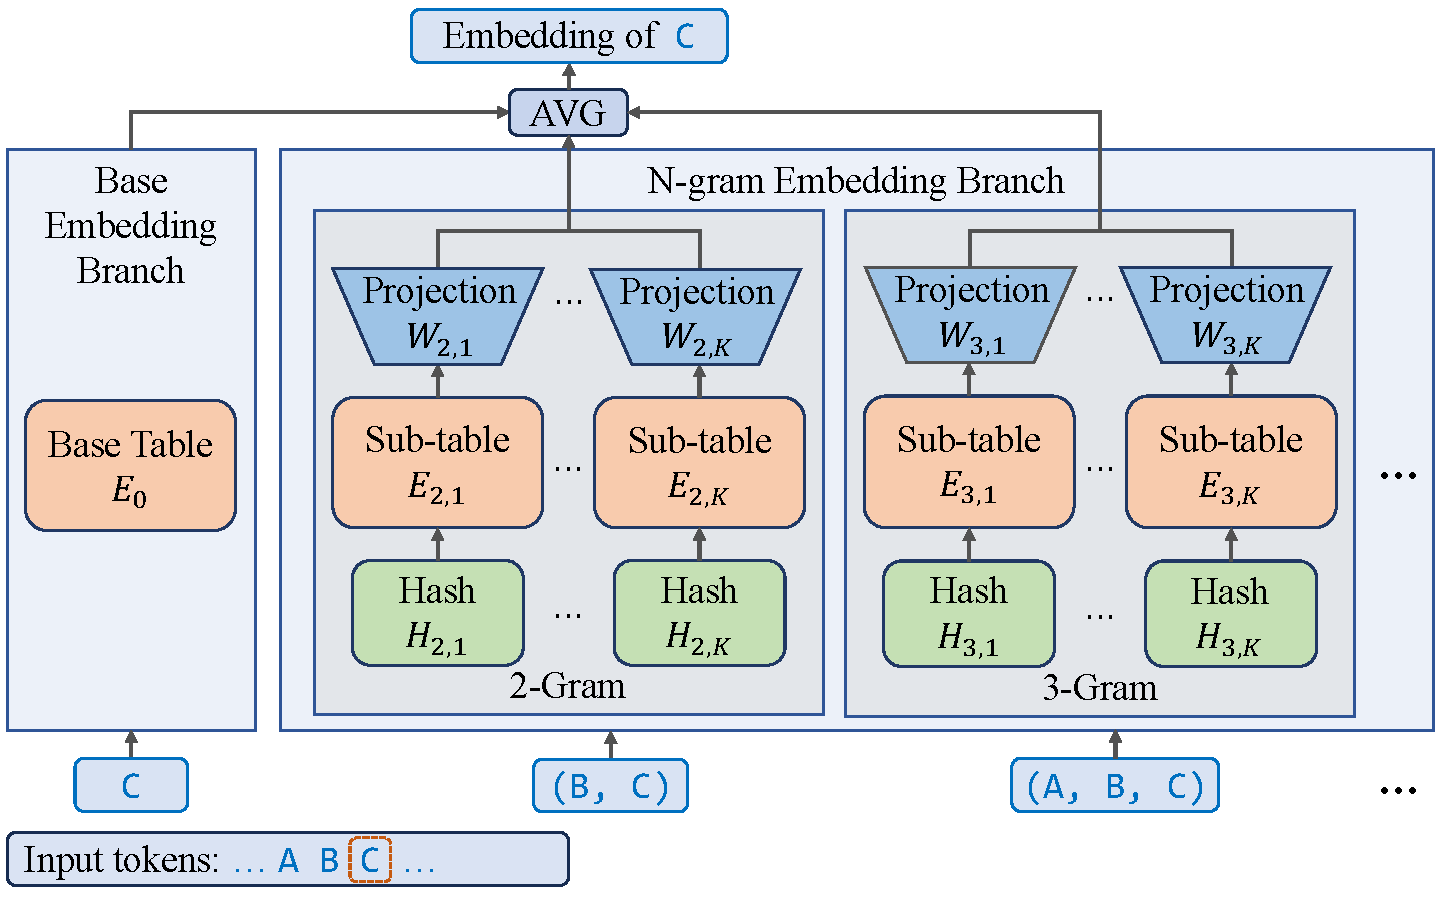
\includegraphics[width=1.0\linewidth]{figures/ngram_embedding_layer.pdf}
    \caption{Architecture of an \textit{n}-gram embedding layer. The token
    embedding is augmented with hashed \textit{n}-gram embedding branches.
    Figure from \citep{liu2026scalingembeddingsoutperformsscaling}.}
    \label{fig:ngram-embedding-layer}
\end{figure}
Some solutions exist to augment the LLM memory without the complexity
and cost of searching a large key-value store.
Embedding memory layers can be seen as a special case of sparse key-value memory
layers, where the keys are not learned dense vectors but fixed discrete indices.
For a standard embedding table, the key is simply the token index, and the value
is the corresponding embedding vector. During the forward pass, each token
$x_i$ maps to exactly one index. In that sense, the retrieval is a TopK with
$K=1$, but without any query-key similarity to compute.
Embedding memory layers are used in several recent LLMs as a simple trick to
augment the model memory without increasing the forward cost too much. A simple
version appears in the modded-nanoGPT speedrun as \textit{value embeddings} where   
extra token embeddings are summed with the value vectors in the attention
layers.\footnote{
    \url{https://github.com/KellerJordan/modded-nanogpt}
}
More generally, the embedding table can store not only token embeddings, but also
\textit{n}-gram embeddings
\citep{roy2022ngrammeraugmentingtransformerslatent,liu2026scalingembeddingsoutperformsscaling}
to augment the model memory.
This approach is used and has been studied in many architectures, including
LongCat-Flash~\citep{liu2026scalingembeddingsoutperformsscaling} and Qwen3.8-Flash-Next
\footnote{
    \url{https://github.com/QwenLM/Qwen3.8-Flash-Next/blob/main/tech_report.pdf}
}
Figure~\ref{fig:ngram-embedding-layer} shows how n-gram embeddings are used in
LongCat-Flash-Lite. The embedding memories are used only in the input embedding
module, before the Transformer layers. For each token position $i$, the model
forms left-context n-grams ending at the current token, such as $(B,C)$ or
$(A,B,C)$. These n-grams are mapped through hash functions to embedding tables.
The retrieved unigram and n-gram embeddings are projected when needed, averaged,
and used as the initial hidden representation $x_i^{(0)}$ passed to the
Transformer stack.

There are several ways to inject embedding-memory information into a Transformer
architecture. LongCat-Flash-Lite \citep{liu2026scalingembeddingsoutperformsscaling} 
uses it to construct the input token representations for the Transformer backbone.
Qwen3.8-Flash-Next instead injects the retrieved n-gram vectors inside the
Transformer, at a selected layer.
The authors found that when the n-gram vocabulary is
scaled by adding extra parameters, loss decreases monotonically, while downstream
performance stagnates, as shown in Table~\ref{tab:qwen-ngram-vocab-scaling}.

\begin{table}[!ht]
    \centering
    \footnotesize
    \setlength{\tabcolsep}{4pt}
    \begin{tabular}{lcccccc}
        \toprule
        & & \multicolumn{3}{c}{\textbf{Knowledge}} & \multicolumn{2}{c}{\textbf{STEM}} \\
        \cmidrule(lr){3-5} \cmidrule(lr){6-7}
        \textbf{Vocab. Scale} & \textbf{Loss} & \textbf{MMLU} & \textbf{MMLU-Pro} & \textbf{SuperGPQA} & \textbf{MATH} & \textbf{GSM8K} \\
        \midrule
        None & 1.585 & 62.78 & 33.43 & 20.97 & 32.52 & 59.21 \\
        $20\times$ & 1.553 & 64.14 & 34.46 & 21.83 & \textbf{37.38} & \textbf{65.09} \\
        $50\times$ & 1.541 & 64.71 & 35.80 & 21.49 & 37.32 & 64.00 \\
        $100\times$ & 1.534 & 64.70 & \textbf{35.87} & \textbf{21.93} & 36.98 & 63.08 \\
        $200\times$ & \textbf{1.526} & \textbf{64.85} & 35.21 & 21.11 & 35.34 & 62.96 \\
        \bottomrule
    \end{tabular}
    \caption{Effect of \textit{n}-gram vocabulary scaling in Qwen3.8-Flash-Next.
    Vocabulary scales are measured relative to the base tokenizer vocabulary
    size. Larger vocabularies add parameters. Table adapted from
    \citep{qwen2026qwen38next}.}
    \label{tab:qwen-ngram-vocab-scaling}
\end{table}

\subsection{Post-training Activation Sparsity}
We presented several approaches that induce activation sparsity during training,
but sparsity can also be introduced after pre-training. These post-training
activation-sparsity methods are used to reduce the inference cost of dense
pre-trained LLMs.

Most modern LLMs use gated MLPs with smooth activation functions such as GELU,
SiLU, or Swish, which produce few exact zeros. A natural way to recover
activation sparsity is therefore to replace, after training, these smooth activations with
ReLU-like activations. This process is called \textbf{ReLUfication}\citep{mirzadeh2023relustrikesbackexploiting}. In gated
MLPs, this makes parts of the intermediate activation exactly zero, so the
corresponding intermediate channels in the up and down projections can be skipped
during inference. However, directly changing the activation function creates a
distribution shift in the pre-trained model, so additional calibration or
continued training is usually needed to recover performance.

Instead of replacing the MLP activation function, other approaches exploit
the fact that many intermediate activations are concentrated near zero and can
therefore be sparsified by magnitude thresholding. TEAL~\citep{TEAL} applies training-free
magnitude pruning to input activations of the MLP, using layer-dependent
thresholds estimated from calibration data. 
CATS~\citep{lee2024cats} thresholds the absolute value of the gate activation
$\mathrm{SiLU}(xW_{\mathrm{gate}})$ and sets small values to zero. The resulting
mask makes it possible to skip the corresponding channels in the up and down
projections during inference, improving latency. Learn-To-be-Efficient (LTE) proposes
a training-aware approach to learn sparsity via sigmoid-router
thresholding~\citep{zheng2024learntobeefficient}.

There are also approaches that transform dense pre-trained models into MoEs.
\textbf{MoEfication} is a method for converting dense FFN layers into routed experts,
while \textbf{upcycling} more generally means initializing an MoE from one or several
dense checkpoints and then continuing training. For example, Qwen1.5-MoE-A2.7B
is upcycled from Qwen-1.8B, and Qwen2 extends this line with a larger MoE
model~\citep{qwen2024qwen15moe,qwen2}. Combining several dense models is not
trivial, because their layers, notably attention layers, can differ a lot.
Several studies therefore focus on how to combine different dense models into an MoE. 
BAM~\citep{zhang2024bamjustlikethat} proposes to reuse both
FFN and attention parameters from dense models, using a mixture-of-attention
variant. Nexus studies a continual domain-adaptation setting, where new domain
experts are added to an existing MoE using an adaptive router initialized from
domain embeddings~\citep{gritsch-etal-2025-nexus}.

\subsection{Matryoshka Learning}

\begin{figure}[!t]
    \centering
    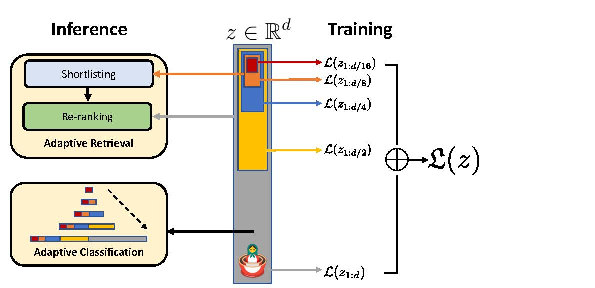
\includegraphics[width=\linewidth]{figures/mrl_figure1.pdf}
    \caption{Matryoshka Representation Learning trains a representation to be
    useful at several embedding dimensions. Figure adapted from \citep{MRL}.}
    \label{fig:mrl-figure1}
\end{figure}

Activation sparsity reduces the number of parameters used for each token, 
but it does not reduce the memory footprint of the model,
since the full model parameters must be hosted in memory. 
Another approach is \textbf{Matryoshka Learning}, where a single model is
trained to nest multiple model or embedding sizes within it. At inference time,
it is possible to use the embedding dimension or model size that fits the
compute and memory budget.
The idea first emerged in representation learning as \textbf{Matryoshka
Representation Learning} (MRL)~\citep{MRL}. Given a set of target embedding
dimensions $\mathcal{D} = \{d_1, d_2, \ldots, d_m\}$, MRL trains these
dimensions jointly by summing the task loss over the different representation
sizes: $\mathcal{L}_{\mathrm{MRL}} = \sum_{d \in \mathcal{D}} \mathcal{L}\left(y, f_{d}(x)\right)$
where $x$ is the full representation and $f_d$ selects or projects it to a
$d$-dimensional representation. Most of the time, this function is simply a slicing operation
that selects the first $d$ dimensions of the representation, but it can also be a learned projection. 
The MRL framework is illustrated in Figure~\ref{fig:mrl-figure1} and
is widely used in retrieval models. It helps reduce the disk usage of the embedding
store, and allows a trade-off between retrieval speed and accuracy.
MRL can be seen as a form of activation sparsity since slicing a vector $x_{[:d]}$
means implicitly setting the remaining dimensions $x_{[d:]}$ to zero.


\begin{figure}[!t]
    \centering
    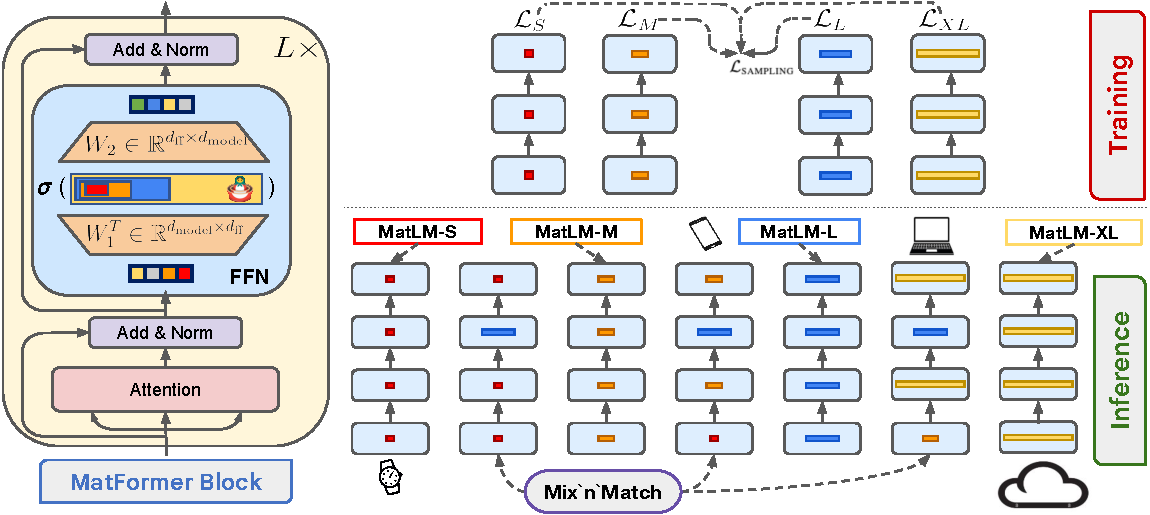
\includegraphics[width=\linewidth]{figures/matformer_figure1.pdf}
    \caption{MatFormer nests several FFN sizes inside the Transformer block and
    trains the corresponding submodels jointly. Figure from
    \citep{devvrit2024matformer}.}
    \label{fig:matformer-figure1}
\end{figure}

More recent work extends the same principle to LLM architectures. 
These methods train nested Transformer submodels of different sizes 
inside a larger model~\citep{devvrit2024matformer}. This design is used in
Gemma~3n E2B and E4B\footnote{\url{https://developers.googleblog.com/en/introducing-gemma-3n-developer-guide/}.}
and Gemma~4 E2B and E4B.\footnote{\url{https://ai.google.dev/gemma/docs/core/model_card_4}.}
At inference time, it is possible to select a submodel of the desired size
depending on the compute and memory budget.



\section{Our contribution to activation sparsity}
Our contributions examine the limitations of fixed representation
sizes and explore more adaptive sparsity:
\begin{enumerate}
    \item We study Matryoshka Representation Learning (MRL) across speech
    and text. We show that MRL doesn't achieve optimal sparsity,
    as Matryoshka embeddings concentrate information
    in relatively few components, leaving the remainder unused.
    This suggests scope for more effective sparsity than fixed prefix slicing.

    \item In a preliminary study, still ongoing at the time of writing,
    we explore \textbf{ZeroNeuron}, an adaptive, fine-grained,
    differentiable activation-sparsity mechanism for MLP activations and
    embedding representations. ZoN follows the same motivation as fine-grained
    MoEs and sparse memory layers: a larger hidden representation can be used,
    but only a subset of coordinates should be active for each input
    token~\citep{krajewski2024scaling,lample2019largememorylayersproduct,
    he2024mixturemillionexperts}. However, unlike TopK-based MoE routing or
    memory lookup, ZoN does not select a fixed number of experts or retrieve
    a subset of keys through explicit routing; instead, it learns a pointwise
    gate over the intermediate coordinates of the dense MLP. This preserves the
    dense tensor-parallel communication pattern while allowing the level of
    sparsity to vary with the input, which is the key difference from
    discrete expert routing and memory retrieval
    methods~\citep{huang2024hardertasksneedexperts,
    wang2025remoefullydifferentiablemixtureofexperts,
    huang2025ultrasparsememorynetwork}. ZeroNeuron realizes a communication-
    efficient form of adaptive activation sparsity directly in the standard
    MLP computation.
\end{enumerate}
